\documentclass{article}
\usepackage[french]{babel}
\usepackage[utf8]{inputenc}
\usepackage[T1]{fontenc}
\usepackage{microtype}
\usepackage{subcaption}
\usepackage{csquotes}
\usepackage{float} % Ajoute ce package dans le préambule
\usepackage{hyphenat}
\usepackage{graphicx}
\usepackage[hidelinks]{hyperref}
\usepackage[backend=biber,style=ieee,sorting=nyt]{biblatex}
\usepackage[a4paper, left=3cm, right=3cm, top=3cm, bottom=3cm]{geometry}
\usepackage{fancyhdr}
\usepackage{xcolor}
\usepackage{hyperref}
\usepackage{listings}
\usepackage[normalem]{ulem}
\usepackage{amsmath} % dans le préambule
\usepackage{tcolorbox} % dans le préambule
\usepackage{xcolor} % Pour la coloration syntaxique
\usepackage{setspace} % Pour l'interligne
\onehalfspacing %interlignes


\lstdefinestyle{mystyle}{
  backgroundcolor=\color{gray!10},
  basicstyle=\ttfamily\small,
  frame=single,
  breaklines=true,
  captionpos=b,
  keywordstyle=\color{blue},
  commentstyle=\color{gray!70!black},
  stringstyle=\color{teal},
  language=Python,
}
\lstset{style=mystyle}

\newif\ifconfidentiel
\confidentielfalse  % <-- active le mode confidentiel

\newif\ifshowcomments
\showcommentstrue  % <-- active les commentaires
%\showcommentsfalse  % <-- désactive les commentaires

\ifshowcomments
  \newcommand{\commentaire}[1]{\textcolor{red}{\textbf{[Commentaire: #1]}}}
  \newcommand{\shana}[1]{\textcolor{blue}{\textbf{[Shana: #1]}}}
  \newcommand{\todo}[1]{\textcolor{orange}{\textbf{[À faire: #1]}}}
\else
  \newcommand{\commentaire}[1]{}
  \newcommand{\shana}[1]{}
  \newcommand{\todo}[1]{}
\fi
\addbibresource{bibliography.bib}

\begin{document}

\begin{titlepage}
    \begin{center}
        
        \begin{figure}[H]
            \centering
            \begin{minipage}[c]{0.45\textwidth}
                \centering
                \includegraphics[width=1\textwidth]{images/logo_paris_saclay.png}
            \end{minipage}
            \hfill
            \begin{minipage}[c]{0.45\textwidth}
                \centering
                
\includegraphics[width=1\textwidth]{images/logo_kappasante.jpg}
            \end{minipage}
        \end{figure}
   

        {\Large \textbf{Université d'Évry Paris-Saclay}}\\[0.5cm]
        {\Large \textbf{Mémoire de Master MIAGE}}\\[2cm]

        {\huge \textbf{Dans quelles mesures les technologies IoT des voitures peuvent-elles être adaptées pour répondre aux besoins spécifiques de la sécurité des motos sur les routes ? }}\\[1cm]
        {\Large\textbf{Année universitaire :}} \\[0.5cm]
        {\Large \textbf{2024/2025}}\\[1cm]
        {\Large \textbf{Shana LEFEVRE}}\\[2cm]
        {\Large Maître d'apprentissage: \textbf{Clément LECLERCQ}}\\[0.5cm]
        {\Large Tutrice enseignante: \textbf{Farida ZEHRAOUI}}\\[3cm]
        {\Large{4 rue Cléry, 75002 Paris}} \\
        {\Large{23 Bd François Mitterrand, 91000 Évry-Courcouronnes}} \\[0.5cm]
    \end{center}
\end{titlepage}


\tableofcontents % Table des matières

%inclusion des différents chapitres
\newpage
\section{Remerciements}
Je tiens tout d'abord à remercier toutes les personnes qui m'ont soutenue et accompagnée tout au long de mon parcours académique et professionnel. 
Je remercie tout particulièrement: \
\begin{itemize}
    \item \textbf{Monsieur Clément Leclercq }, mon maître d'apprentissage, pour sa confiance, son accompagnement et ses conseils tout au long de mon année d'apprentissage.
    \item \textbf{Madame Farida Zehraoui}, ma tutrice enseignante, pour son encadrement et ses conseils.
    \item \textbf{Monsieur Hichem Arioui}, Vice-Président Relations Internationales et Innovation, pour m'avoir ouvert ses portes de son laboratoire afin que je puisse effectuer mes recherches.
    \item \textbf{Mes collègues du département informatique : Monsieur David Clément, Monsieur Mathieu Le Hoang et Monsieur Thibaud Caron}, pour leur soutien, leur bienveillance et leur aide précieuse tout au long de mon apprentissage.
    \item \textbf{Monsieur Christophe Brunat}, directeur informatique, pour son accueil et sa disponibilité.
    \item \textbf{Ma famille}, pour leur soutien et leurs encouragements tout au long de mon parcours.
\end{itemize}
Je remercie également mes collègues de l'entreprise Kappa Santé pour leur accueil chaleureux et leur soutien tout au long de mon apprentissage. Leur expertise et leur bienveillance ont été des atouts précieux dans mon parcours.
\newpage
\section{Fiche de bilan et de syntèse}
\subsection{Présentation de l'activité en entreprise}
\subsubsection{L'entreprise d'accueil}
L’entreprise Kappa Santé a été créée en 2003 par Mr SCHÜCK (médecin de
santé publique) et par Mme TEXIER (pharmacienne) en vue d’apporter des
services de qualité. Avec une expertise ciblée sur les domaines de:
l’épidémiologie, pharmaco- épidémiologie, la constitution d’e-cohortes i et des
interventions en santé publique et numérique, cette société répond aux
demandes à la fois au niveau national et européenne.
Cette CRO (Contract Research Organization) est une SAS (Société Anonyme
Simplifiée) au capital de 50 000 €.
Le siège social de l’entreprise est situé au 4 rue Cléry à Paris, dans le 2e
arrondissement.
Kappa Santé est membre de l’ENCEPP (European Network of Centres for
Pharmacoepidemiology and Pharmacovigilence), de l’AFCROs (association de
CRO) et du pôle compétitivité numérique Cap digital (collectif européen
d’innovateurs).
L’entreprise Kappa Santé est l’entreprise mère de Kap Code depuis 2015. Kap
Code est une entreprise qui récupère des données liées à la santé sur les
réseaux sociaux.
En mars 2023, Kappa Santé a été racheté par Apices, une entreprise CRO
espagnole qui réalise des études cliniques.
À ses débuts, Kappa Santé réalisait des études dans le but de recueillir des
informations sur des médicaments mais depuis 2012, la société s’est diversifiée
et elle est devenue polyvalente en proposant des services comme le suivi et le
monitoring, la création de protocole, ...
De grosses entreprises comme Pfizer, Janssen, AstraZeneca, Microsoft, IBM... font confiance à Kappa Santé. Les principaux concurrents de Kappa Santé sont
Aixial, Axonal, Cemka, Clinact, Euraxi, Icon, Icta, Iqvia, Sanoïa...

L’équipe dont je fais partie intègre le Département Informatique où M. BRUNAT est le directeur informatique.
Nous développons en Java à l’aide du Framework JSF (Java Server Faces) et
des composants PrimeFaces.
\begin{figure}[H]
    \centering
    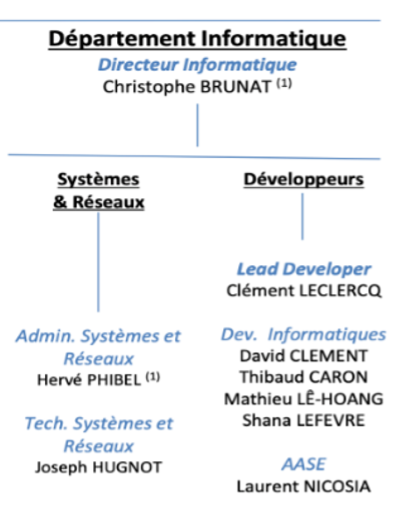
\includegraphics[width=0.4\textwidth]{fiche_bilan/fiche_bilan_images/organigramme_info.png} 
    \caption{Organigramme de l'entreprise}
\end{figure}
Pour communiquer avec notre base de données (développeur), JPA définit des
entités qui sont une instance de classe et nous permet d’écrire des
programmes qui interagissent avec la base de données.
\begin{figure}[H]
    \centering
    \includegraphics[width=0.3\textwidth]{fiche_bilan/fiche_bilan_images/intégration_jpa.png} 
    \caption{Schéma d'intégration de JPA}
\end{figure}

\subsubsection{Le maître d'apprentissage}
Notre équipe est composée de cinq développeurs dont un « lead developer »,
Monsieur Clément LECLERCQ (voir schéma précédent), c’est notre superviseur. Il prend des décisions, supervise les projets, mène et assiste des réunions afin de représenter l'équipe des développeurs. Monsieur Clément LECLERCQ est également mon maître d’apprentissage. Il développe également sur les projets.
Notre objectif est d’assurer le développement et la maintenance de tous nos outils informatisés de recueil de données en utilisant des langages et des outils
de développement.
\subsubsection{Résumé des travaux proposés par l'entreprise}
L'intitulé de mon contrat d'apprentissage est « Développeur Java ».
\begin{figure}[H]
    \centering
    \includegraphics[width=0.8\textwidth]{fiche_bilan/images/Capture d’écran 2025-07-30 à 09.38.36.png} 
    \caption{Schéma chronologie d'un projet}
\end{figure}
Mon activité principale est de développer et d’entretenir des applications
\(electronic Case Report Forms\). Ces formulaires permettent de collecter des données cliniques de manière structurée et sécurisée. Ils sont utilisés dans le cadre d'études cliniques pour recueillir des informations sur les patients, les traitements administrés, et les résultats obtenus. Mon rôle consiste à développer ces e-CRF en respectant les spécifications fournies par les chefs de projet et les Data Managers, tout en assurant leur bon fonctionnement et leur conformité aux exigences réglementaires.\
Pour développer des études, nous partons d'une application dites "starter" qui
permet de créer un e-CRF. Cette application est une sorte de modèle qui nous
permet de créer un e-CRF. Nous la faisons évoluer en fonction des
besoins de l'étude. Les dead-line varient en fonction de la taille de l'étude et de la
complexité de l'e-CRF. 
\subsubsection{Travaux effectués en entreprise}
Mon activité au sein de l’entreprise est de développer et d’entretenir des
applications, des
formulaires en ligne nommés de e-CRF.
Tout au long de l’année, j’ai poursuivi mon apprentissage dans le
développement en utilisant les Bonnes Pratiques de développement de Kappa
Santé.
Pour mener à bien notre projet, nous travaillons avec un chef de projet ainsi
qu’avec un Data Manager.
Cette année, j’ai épaulé mes collègues sur leurs projets en développant
diverses fonctionnalités :
\begin{itemize}
    \item Création d’envoi mails automatiques aux utilisateurs : automatiser l’envoi
    de mails en fonction des évènements qui se passent sur l’application, par
    exemple, l’insertion d’un
    patient par un utilisateur, un récapitulatif quotidien des évènements
    indésirables...
    \item Résolution de bugs, à la suite d’une demande sur notre logiciel Redmine,
    \item Réalisation des Phases Listener : C’est un outil propre à JSF (Java Server
    Faces). C’est une interface implémentée par des objets notifiés sur le début
    ou la fin d’un traitement,
    d’un cycle. Ainsi, nous pouvons personnaliser le comportement de nos e-
    CRF. La principale utilisation des Phase Listener est de vider les sous-
    champs entre les pages. On s’en sert pour vider les sous-champs entre les
    pages.
    \item Implémentation des contrôles bloquants et non-bloquants : Ce sont des
    contrôles qui permettent de savoir si la donnée correspond aux attentes du
    e-CRF. Un contrôle bloquant nécessite que l’utilisateur corrige la donnée non-conforme avant
    de pouvoir passer à la page suivante du questionnaire. En revanche, pour
    un contrôle non-bloquant, un message avertit simplement l’utilisateur de la
    non-conformité avant qu’il ne puisse continuer. Tous ces contrôles sont spécifiés dans le document « Data Validation Plan », qui contient toutes les
    instructions nécessaires à la réalisation des contrôles.
    \item Implémentation des Locked Queries : C’est une fonctionnalité propre à
    Kappa Santé. Ils permettent de bloquer, verrouiller, griser, et rendre
    inaccessible un champ enfant
    lorsque la case parent est cochée. Cette fonctionnalité est précieuse car
    elle évite l’enregistrement de données inutiles dans la base de données.
    Ainsi, l’utilisateur ne peut
    pas entrer des informations dans les champs. Pour faire ces modifications,
    j’utilise le fichier xhtml associé au formulaire avec une condition d’affichage
    « rendered ».
    \item Amélioration de nos outils, de notre starter. Pour cela, des réunions sont plannifiées avec l'ensemble du personnel pour savoir quels sont les points à améliorer à la suite de nos projets. Cela permet de montrer ce projet à des promoteurs pour répondre aux appels d'offres.
\end{itemize}


Mes missions sont également :
Création de fiches de procédures, la participations aux réunions. 
Aujourd’hui après quelques mois au sein de l’entreprise, j’ai mes propres
études. Tout commence par la création de l’étude avec la mise en place tout ce
dont nous avons besoin pour son bon déroulement (base de données…). Au
cours du développement de l’étude, on retrouvera les fonctionnalités vue
précédemment.

\vspace{0.5cm}
Cette année, pour ma dernière année d'alternance, j'ai poursuivi ce que j'ai appris durant ces deux dernières années. J'ai développé deux études pour le même promoteur. Les dead line étaient serrées entre les modifications des e-crf de la part des promoteurs et mes jours en entreprise mais avec un peu d'aide de mes collègues, nous avons pu accomplir cette tâche haut la main. À la suite des retours du chef de projet, nous avons su que le promoteur était très satisfait de notre travail. 
\begin{figure}[H]
    \centering
    \includegraphics[width=1\textwidth]{fiche_bilan/images/Capture d’écran 2025-07-30 à 10.44.02.png} 
    \caption{Planning des projet sur lesquels j'ai pu travailler.}
\end{figure}
Les légendes :\\
- En vert: Le développement des projets,\\
- En bleu: Les phases de tests côté Data Manager,\\
- En orange: Modifications à la suite des retours du promoteur.\\
Lors des périodes creuses sur mes projets, j'épaule mes collègues sur leurs projets, en prenant de l'avance par exemple, en développant des queries ou bien en améliorant nos outils.

%conclusion
\vspace{0.5cm}
Développer en Java au sein de l’entreprise m’a permis également de maîtriser davantage ce langage dans mes projets universitaires. Faire du Java en formation m’a apporté un autre regard sur les applications de Kappa Santé. Ma technique d’approche est différente : plus de lecture, plus de recul pour mieux comprendre l’architecture d’un projet. 
Cette année d’alternance au sein de Kappa Santé a été encore riche tant au niveau professionnel que personnel.
Le cadre de travail et l’équipe dont je faisais partie ont été exceptionnels et j’y ai beaucoup appris. Maintenant, cette vie professionnelle m'enmènera vers de nouveaux horizons.

\newpage
\section{Introduction}
%•	Présentation du sujet et de son importance.
\subsection{Contexte et enjeux}
%Abord IOT
L'IoT\footnote{Internet des objets} a révolutionné de nombreux aspects de notre société: la santé, de l'agriculture à l'industrie 4.0, en passant par les transports et les communications.
Les \textbf{technologies embarquées et connectées} désignent l’ensemble des systèmes électroniques intégrés aux véhicules (voitures et motos) permettant d’améliorer la sécurité, le confort et la connectivité. Ces technologies incluent : les systèmes de communication, les capteurs, les caméras, les radars, les lidars\footnote{Light Detection And Ranging: est un système de mesure qui utilise un faisceau laser pour calculer avec précision la distance d’un objet.}, les systèmes d’aide à la conduite (ADAS\footnote{Advanced Driver Assistance System:désigne l’ensemble des technologies embarquées dans un véhicule destinées à améliorer la sécurité, le confort et l’efficacité de conduite. }) et les plateformes de gestion des données.\\
%enjeux -> sécurité routière
L’accidentalité routière en France reste un enjeu majeur de sécurité publique, avec des milliers d’accidents chaque année causant des pertes humaines et matérielles importantes. Malgré les avancées en matière de prévention et de réglementation, les comportements à risque et les conditions de circulation continuent d’alimenter cette problématique.
En France, il y a environ 2,3 à 2,5 millions de motards\cite{actiEouteNbMotardFr}, ce qui représente 2\%  du trafic.
Le document\cite{la_securite_routiere_accidentalite_2024} fournit des informations et des statistiques sur les accidents de la route. Les données définitives datent du 31 mai 2024.

\begin{figure}[h]
    \centering
    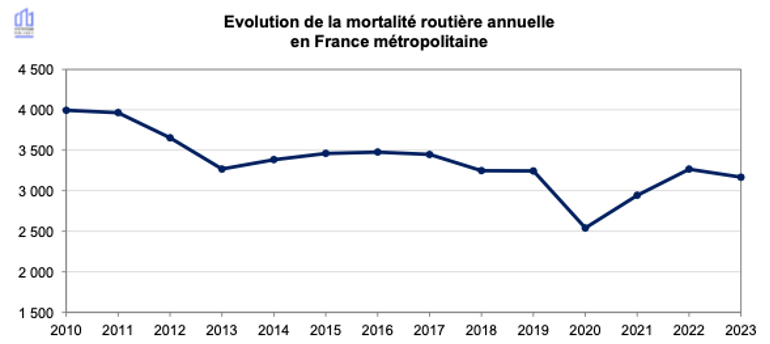
\includegraphics[width=0.8\textwidth]{images/evolution_mortalite_securite_routiere_france.png} 
    \caption{ONISR données relatives aux accidents corporels enregistrés par les forces de l'ordre en France métropolitaine.}
\end{figure}

Grâce au graphe précédent, on constate qu’il y a une diminution sensible du nombre d’accidents mortels sur la dernière décennie surtout entre 2011 et 2013. Différents paramètres expliquent cette évolution : nouvelles infrastructures routières, les dernières technologies de sécurité (casques, ABS…), les renforcements de la règlementation, mise en place de radars et nombreuses campagnes de sensibilisation… L’ensemble de ces éléments ont contribué à réduire la mortalité bien que chaque année, on enregistre, encore, autour de 3500 morts sur les routes tous véhicules confondus. 

\begin{figure}[H]
    \centering
    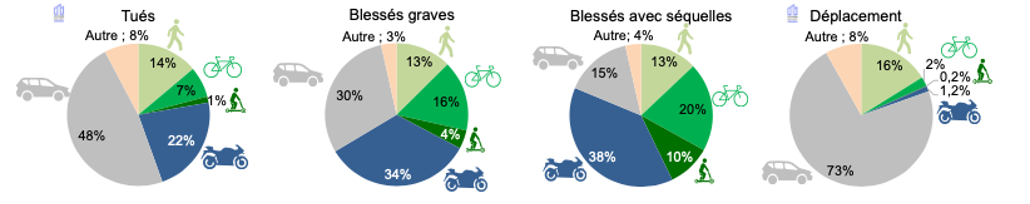
\includegraphics[width=0.9\textwidth]{images/camambert_accidents_differents_vehicules.png} 
    \caption{ONISR Données relatives aux accidents corporels enregistrés par les forces de l'ordre, en France métropolitaine.}
\end{figure}

Concernant les accidents corporels et de mortalité sur la route, les conducteurs de deux-roues sont les plus impactés. Le conducteur n’étant pas protégé par une carrosserie, il est plus vulnérable en cas d’accident. Le motard doit s’équiper de façon rigoureuse afin de limiter les blessures corporelles causées par le choc.\\
%enjeux -> technologies
C'est un défi majeur pour les autorités et les constructeurs de véhicules de trouver des solutions pour réduire le nombre d'accidents et améliorer la sécurité des usagers de la route, en particulier des motards. Les technologies IoT offrent des opportunités pour répondre à ces enjeux en améliorant la détection des obstacles, la perception environnementale, l'aide à la conduite et l'analyse des données pour une meilleure prise de décision.\\


\subsection{Définitions et concepts clés}
%••	IoT (Internet des Objets) appliqué aux transports.
Qu'est-ce que l'IoT ?\\
L'IoT est un réseau d’objets physiques connectés à Internet qui sont capables de collecter et d’échanger des données en temps réel. Ces objets peuvent être des capteurs, des appareils domestiques intelligents, des équipements industriels, des véhicules et bien plus encore. Ils font face à des défis et des enjeux importants comme l'exposition aux menaces de cyberattaques, l'uniformité des systèmes pour leur bon fonctionnement, la consommation d'énergie et enfin, le respect aux droits privés. \\
• \textbf{Les capteurs et caméras} : détectent les obstacles, surveillent l’environnement et assistent à la conduite (ex. : radars, lidars, caméras 360°). Selon dDruid\cite{capteur} un capteur IoT est un "composant électronique qui transforme les variations physiques ou environnementales en signaux électriques exploitables pour surveiller, contrôler ou interagir avec des systèmes connectés".
Les principaux types de capteurs d'IoT sont: les capteurs de température et d'humidité, les capteurs de mouvement et de présence, les capteurs de lumière et de luminosité, les capteurs de gaz et de qualité de l’airCapteurs de pression et de force et enfin les capteurs de proximité et de distance.
\begin{figure}[H]
    \centering
    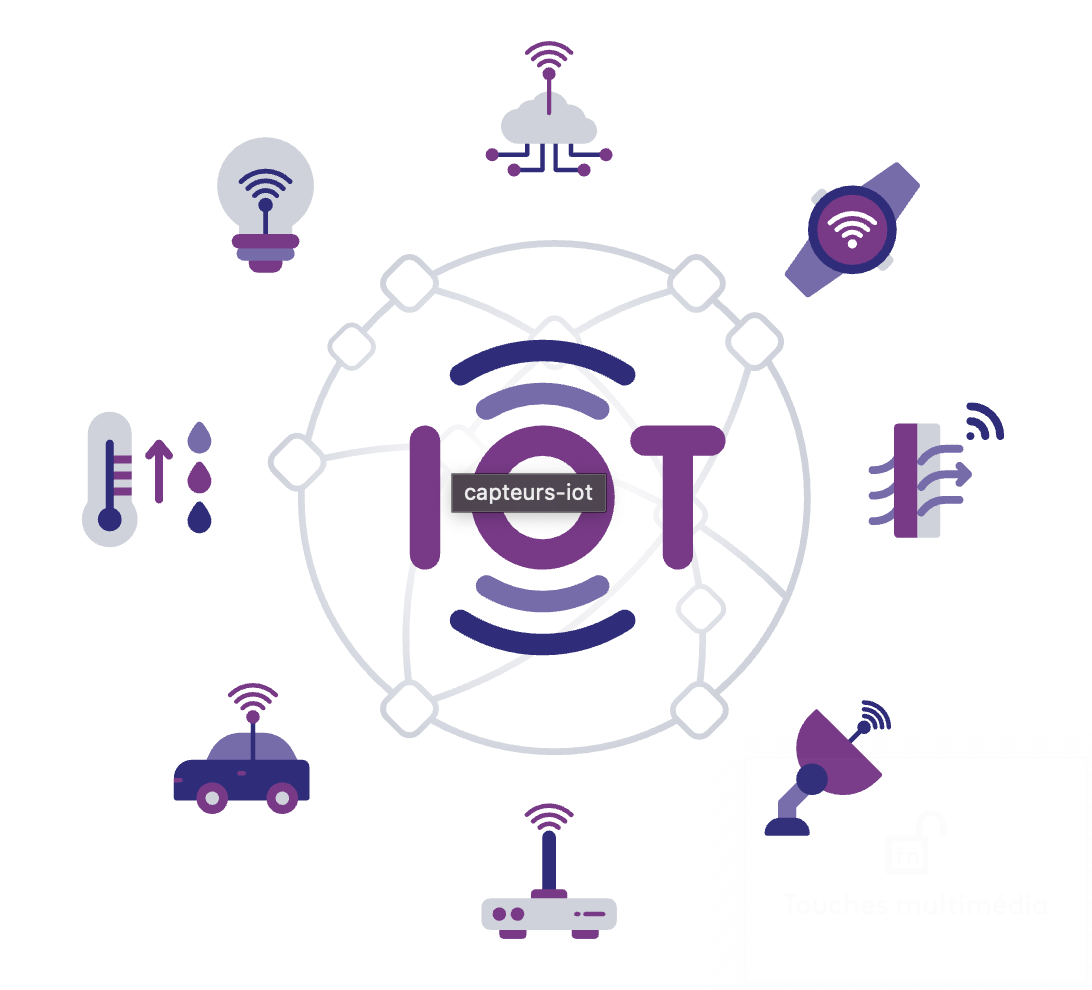
\includegraphics[width=0.7\textwidth]{images/capteur.png} 
    \caption{Intéraction des capteurs}
\end{figure}
Ils fonctionnent de manière autonome tout intégrant des réseaux connectés. Les éléments à identifier en premier lieu sont donc : leur taille, leur consommation d’énergie, leur capacité de traitement local, leur autonomie, leur capacité de communication.\\
• \textbf{Les systèmes d’aide à la conduite (ADAS)} : aident le conducteur en régulant la vitesse, le freinage d’urgence ou le maintien de trajectoire.\\
• \textbf{Les modules de connectivité (4G, 5G, Wi-Fi, Bluetooth)} : permettent l’échange de données en temps réel entre le véhicule et d’autres systèmes, comme les infrastructures routières ou les smartphones.\\
• \textbf{Les plateformes de gestion des données} : traitent les informations collectées pour fournir des services comme la navigation intelligente, l’alerte trafic ou la maintenance prédictive.\\
Ces technologies sont essentielles pour le développement des véhicules intelligents et autonomes, ainsi que pour renforcer la sécurité des motards, souvent plus vulnérables sur la route.
\vspace{0.5cm}

Les \textbf{communications V2V (e) et V2I (Vehicle-to-Infrastructure)} font partie des technologies de transport intelligent (ITS)\footnote{infrastructure technology services} qui permettent aux véhicules et aux infrastructures routières comme les feux de signalisation, les panneaux d’échanger des informations en temps réel.

\begin{figure}[H]
    \centering
    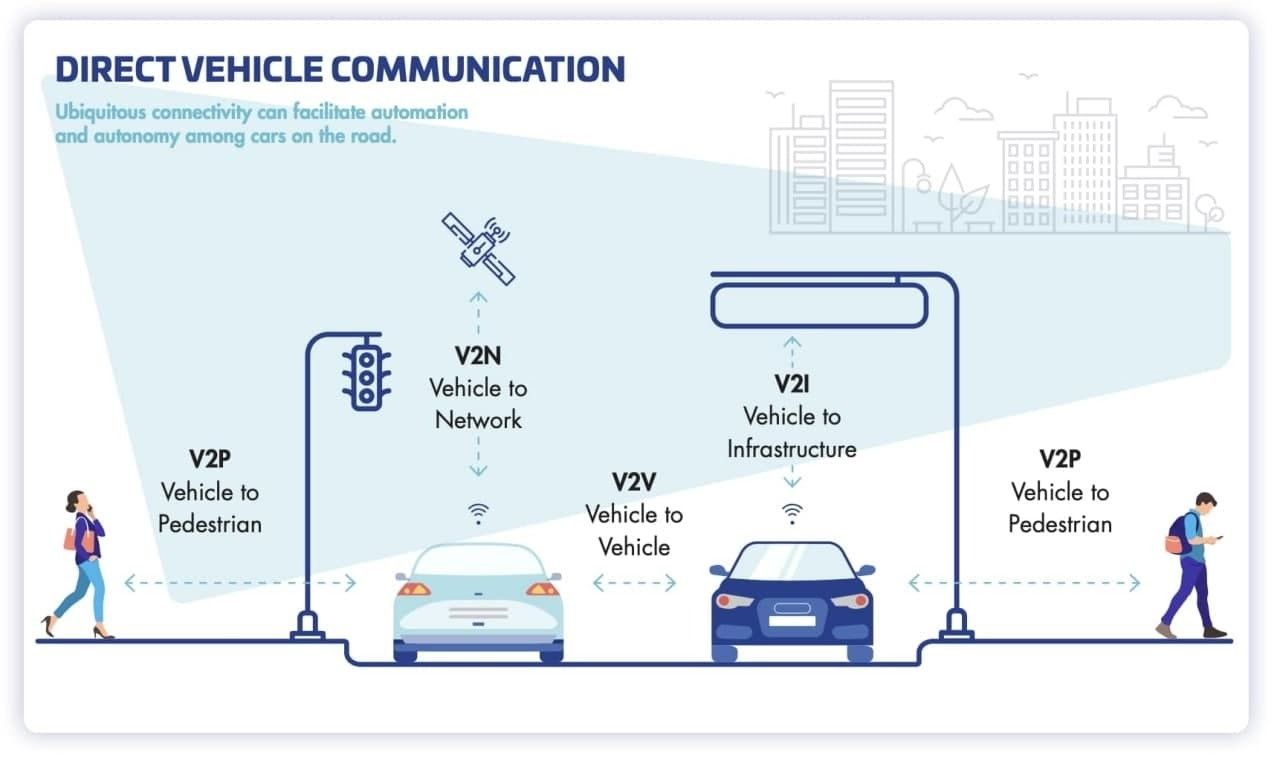
\includegraphics[width=0.7\textwidth]{images/schema_v2.png} 
    \caption{La communication V2X}
\end{figure}

Cette communication offre des mises à jour en temps réel sur les conditions de circulation, les accidents, la météo et la disponibilité des places de stationnement, améliorant ainsi la sécurité et l’efficacité des trajets\cite{joberty_blog}.\\

\newpage
\section{État de l'art}


\subsection{Les technologies IoT dans les voitures}

\commentaire{introduction}
Selon l’entreprise Objenious \cite{noauthor_revolution_2025}, l’Internet des Objets (IoT) constitue une révolution dans l’industrie automobile en rendant les véhicules plus intelligents et connectés. Depuis l’introduction de la norme européenne eCall en 2018, qui impose un système d’appel d’urgence automatique, les constructeurs ont intégré des technologies IoT pour développer des services innovants. Grâce aux réseaux haut débit comme la 4G et la 5G, les véhicules peuvent désormais collecter, envoyer et recevoir des données en temps réel, interagissant ainsi avec les infrastructures routières, les autres véhicules et les usagers.\\
Le marché mondial de l’IoT dans le secteur automobile, estimé à 115,37 milliards de dollars en 2022, devrait atteindre 975,66 milliards de dollars d’ici 2032, avec un TCAC\footnote{Taux de Croissance Annuel Composé : C’est un indicateur qui permet de mesurer la croissance moyenne d’un marché, d’un chiffre d’affaires ou d’un investissement sur plusieurs années, en tenant compte de l’effet cumulatif d’une année sur l’autre.} de 23,8 \% sur cette période \cite{noauthor_taille_2023}.\\
L’intégration des technologies IoT dans les véhicules permet une communication en temps réel entre les véhicules eux-mêmes, les infrastructures et d’autres dispositifs externes. Cette connectivité vise à améliorer la sécurité, l’efficacité et l’expérience de conduite. Les capteurs embarqués collectent et échangent des données sur les conditions de circulation, la météo, les performances du véhicule et le comportement du conducteur. Ces informations sont exploitées pour la maintenance prédictive, la navigation intelligente et l’optimisation des systèmes de conduite autonome.\\
Par ailleurs, la connectivité IoT facilite l’intégration des smartphones et autres appareils avec les véhicules, offrant ainsi des services tels que la surveillance à distance, le suivi des véhicules et des fonctionnalités d’infodivertissement personnalisées. Ces avancées technologiques redéfinissent le secteur automobile, ouvrant la voie à une mobilité plus sûre, plus intelligente et plus autonome.


\subsubsection{Systèmes de communication et d’échange de données}
\todo{A DÉVELOPPER ?}
"Depuis longtemps une voiture collecte des données, ces données sont collectées via les capteurs et traitées par les calculateurs du véhicule." par Innovauto \cite{donnees_echange}.\\
Les différentes données émisent par un véhicule peuvent être \textbf{techniques} (ex: état de charge de la batterie, autonomie restante ...), \textbf{usage} (ex: trajet, style de conduite...) et \textbf{personnelles} (ex: titulaire de la carte grise, agenda du conducteur,...).
%cycle de vie de la donnée
Un véhicule autonome échange des données avec son environnement, et ces données suivent un cycle de vie comportant plusieurs étapes :
\begin{figure}[H]
    \centering
    \includegraphics[width=0.8\textwidth]{images/schéma_cycle_vie_donneées.png} 
    \caption{Cycle de vie de la donnée}
\end{figure}
Les étapes du cycle de vie des données doivent respecter le RGPD\footnote{Règlement Général sur la Protection des Données : Il établit un cadre juridique unifié pour la collecte, le traitement et la protection des données personnelles au sein de l’Union européenne} sans être spécifiquement adaptées à la pratique automobile. De plus, si des véhicules sont commercialisés, ils doivent se conformer aux normes de chaque pays, telles que le RGPD en Europe, le Cloud Act aux États-Unis, et le PIPL\footnote{ Personal Information Protection Law : C’est la loi chinoise entrée en vigueur le 1er novembre 2021, qui encadre la collecte, l’utilisation, le stockage et le partage des données personnelles.} en Chine. Voici un exemple comparatif :
\begin{table}[H]
\centering
\caption{Comparaison entre le RGPD (Union européenne) et le PIPL (Chine)}
\begin{tabular}{|p{4cm}|p{5cm}|p{5cm}|}
\hline
\textbf{Critère} & \textbf{RGPD (UE)} & \textbf{PIPL (Chine)} \\ \hline
\textbf{Date d'entrée en vigueur} & 25 mai 2018 & 1er novembre 2021 \\ \hline
\textbf{Champ d'application} & Toutes les organisations qui traitent des données personnelles de résidents de l’UE, peu importe leur localisation. & Toutes les organisations qui traitent des données personnelles de résidents chinois, y compris à l’étranger si cela concerne leurs droits et intérêts. \\ \hline
\textbf{Consentement} & Doit être libre, spécifique, éclairé et univoque. & Doit être clair, volontaire et informé, avec un accord explicite requis dans certains cas (par ex. données sensibles). \\ \hline
\textbf{Principes clés} & Licéité, loyauté, transparence, limitation des finalités, minimisation, exactitude, limitation de la conservation, intégrité, confidentialité. & Finalité claire, minimisation, transparence, sécurité, responsabilité, respect des droits individuels. \\ \hline
\textbf{Droits des individus} & Accès, rectification, effacement, limitation, opposition, portabilité des données. & Accès, copie, correction, suppression, limitation, opposition, explication du traitement. \\ \hline
\textbf{Données sensibles} & Traitement soumis à des conditions strictes (santé, biométriques, opinions politiques...). & Nécessite un consentement explicite et des mesures renforcées (santé, biométriques, localisation, données financières...). \\ \hline
\textbf{Transfert international} & Autorisé vers pays disposant d’un niveau de protection adéquat ou via clauses contractuelles types. & Soumis à une évaluation de sécurité par l'autorité chinoise et, parfois, à une autorisation préalable. \\ \hline
\textbf{Sanctions} & Jusqu’à 20 millions € ou 4\% du chiffre d’affaires annuel mondial (le plus élevé des deux). & Jusqu’à 50 millions CNY (\textasciitilde 7 millions €) ou 5\% du chiffre d’affaires annuel. \\ \hline
\end{tabular}
\end{table}
En résumé, bien que le RGPD et le PIPL partagent un objectif commun de protection des données personnelles, leurs approches diffèrent sur plusieurs points, notamment dans la portée territoriale, le rôle des autorités de contrôle et le niveau de centralisation des obligations. Le RGPD se concentre sur la transparence et le consentement explicite, 
tandis que le PIPL intègre des exigences plus strictes en matière de transfert transfrontalier et un contrôle accru de l’État.\\
Les données collectées par les véhicules autonomes sont considérées comme des données personnelles et doivent être protégées conformément à la réglementation en vigueur d'après la Thèse de Nolwen LE GUENNEC\cite{le_gennec_machine_2023}.\\
La connectivité des véhicules autonomes pose également des problèmes de sécurité, notamment la vulnérabilité aux attaques informatiques. Des questions se posent sur la manière de protéger ces systèmes contre de telles menaces. Comment peut-on sécuriser ces informations sensibles face aux cyberattaques ?\\
Les programmes informatiques consomment de l’énergie et l'impact environnemental de ces technologies doit être pris en compte.\\
Grâce à la technologie IoT, les véhicules peuvent échanger des données. Voici les 3 modes de fonctionnement des STI\footnote{Système de Transport Intelligent} :
\begin{itemize}
    \item \textbf{Communication véhicule à véhicule (V2V)} : Les véhicules équipés de l’IoT échangent des informations telles que leur vitesse et leur position. Cette communication permet de signaler des accidents ou des pannes, aidant les conducteurs à anticiper les problèmes de circulation et à se déplacer plus efficacement.
    \item \textbf{Communication véhicule à infrastructure (V2I)} : Les véhicules connectés interagissent avec des éléments d’infrastructure routière comme les feux de circulation, les lampadaires et les caméras. L’analyse de ces données peut conduire à des ajustements tels que la modification des limites de vitesse ou la facilitation du passage des véhicules de secours, améliorant ainsi la sécurité routière pour tous les usagers.
    \item \textbf{Communication infrastructure au véhicule (V2I)} : Les infrastructures routières transmettent des informations aux véhicules à proximité, permettant l’affichage en temps réel de données pertinentes pour les conducteurs.
\end{itemize}

\begin{figure}[H]
    \centering
    \includegraphics[width=0.9\textwidth]{images/schéma_systeme_communication_donnees.png} 
    \caption{Tableau comparatif du système de communication V2X d'Innovauto}
\end{figure}

La technologie basée sur les opérateurs mobiles permet une communication avec un serveur distant, mais ne prend pas en charge directement la communication entre véhicules et infrastructures : 
\begin{itemize}
    \item Le ITS-G5 (Wi-Fi) fonctionne sur la bande 5,9 GHz et permet une communication locale et directe entre les véhicules, les infrastructures et les piétons.
    \item Le C-V2X (Cellular-V2X) combine les deux approches, offrant à la fois une communication via les réseaux mobiles et une communication directe entre les véhicules et infrastructures.
    \item Le C-V2X est la solution la plus complète, intégrant les avantages des réseaux mobiles et de la communication directe, ce qui le rend plus adapté aux véhicules autonomes et à la gestion du trafic intelligent.
\end{itemize}

\subsubsection{Capteurs et perception environnementale}
L'évolution des véhicules intelligents repose sur des systèmes de capteurs avancés et de perception environnementale. "Un capteur IoT est un dispositif qui mesure une ou plusieurs variables physiques de l'environnement et envoie les données à un réseau ou à une plateforme IoT pour une utilisation ultérieure." selon le site de l'entreprise IoT\cite{iot_capteur}.\\
Ces technologies permettent aux véhicules de collecter, d'analyser et d'interpréter en temps réel leur environnement afin d'améliorer leur utilisation.
Les principaux capteurs utilisés sont les caméras, les radars, les lidars et les ultrasons.
Ces données permettent de :\\
- Détecter les pannes. \\
- Alerter les propriétaires en cas de dysfonctionnement. \\
- Optimiser la maintenance. \\
- Simplifier les procédures de réparation. \\
- Gerer les flottes de véhicules. \\

%Par exemple, Lormauto, un constructeur français spécialisé dans le rétrofit de véhicules, utilise la connectivité cellulaire 4G pour optimiser l’expérience utilisateur. Cette technologie permet de transmettre de grands volumes d’informations et de surveiller l’état de santé des véhicules et de leurs batteries en temps réel.

La perception de l'environnement consiste à analyser et à interpréter les données fournies par les capteurs pour prendre des décisions en temps réel. La décision repose sur des algorithmes avancés d'IA\footnote{Intelligence Artificielle} qui permettent de reconnaître les objets, d'anticiper les comportements et de réagir en conséquence. Ces technologies sont essentielles pour la conduite autonome et la sécurité des usagers de la route, y compris les motards.
Pour cela, il faut combiner plusieurs informations :
\begin{itemize}
    \item Détecter et classer les objets,
    \item Éstimer leur vitesse et leur trajectoire,
    \item Anticiper les risques et les collisions,
    \item Améliorer la prise de décision.
\end{itemize}
Les avancées en IA en connectivité comme la 5G et la V2X et en traitement des données continueront d’améliorer la perception environnementale des véhicules permettant ainsi la voie à une mobilité plus sûre.

\subsubsection{Aide à la conduite et systèmes ADAS}
%•Détection des obstacles et freinage automatique.
%•Avertissements de collision et assistance au changement de voie.
Dans un monde où la sécurité routière est une priorité, les systèmes avancés d’aide à la conduite (ADAS) révolutionnent la manière dont les véhicules interagissent avec leur environnement, réduisant ainsi les risques d’accidents et améliorant l’expérience de conduite.
Selon le site du Gouvernement \cite{adas_gouv} "Ces technologies ouvrent la voie à des véhicules de plus en plus automatisés, mais ceux qui en sont équipés ne sont pas des véhicules dits « autonomes ». Les aides à la conduite ne remplacent pas le conducteur et ses obligations. Leur usage s’opère sous la surveillance permanente du conducteur, qui reste responsable de la tâche de conduite et de la maîtrise du véhicule."
\begin{figure}[H]
    \centering
    \includegraphics[width=0.8\textwidth]{images/ADAS_schéma.jpg} 
    \caption{Voiture embarquant des systèmes ADAS\cite{continental_adas}}
\end{figure}


\subsubsection{Analyse des données et prise de décision}
L'entreprise Valeo a conçu un radar Lidar « Scala ». D'après LeParisien \cite{le_parisien_radar_2019}, l'entreprise, en 2020 produit 200 000 exemplaires par an. Cette technologie permet à ce que la voiture conduise sans l'intervention d'un humain.\\
\commentaire{yann lecun}
Les recherches sur l'utilisation et l'interprétation des données recueillies par les capteurs sont au coeur des sujets depuis quelques années. Yann LeCun, précurseur du deep learning\footnote{L'apprentissage automatique.} nous présente l'interprétation et l'utilisation de données recueillies.
Ce graphe ci-dessous présente la relation entre l’écart de position d’une voiture sur la voie et l’angle du volant pour ramener la voiture au milieu. 

\begin{figure}[H]
    \centering
    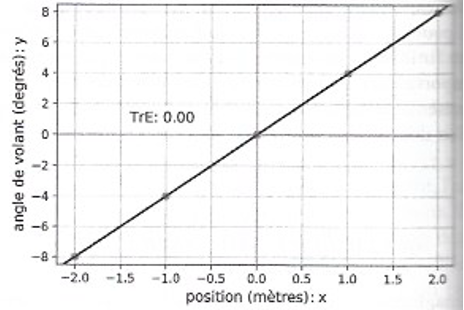
\includegraphics[width=0.7\textwidth]{images/graph1_yannLeCun.png} 
    \caption{Graphe page 88 du livre "Quand la machine apprend".}
\end{figure}
Par exemple, pour une déviation d’un mètre, il faudra incliner le volant de 4 degrés. 
Voici un nouvel exemple de graphique avec de nouvelles données d’entrée :
\begin{figure}[H]
    \centering
    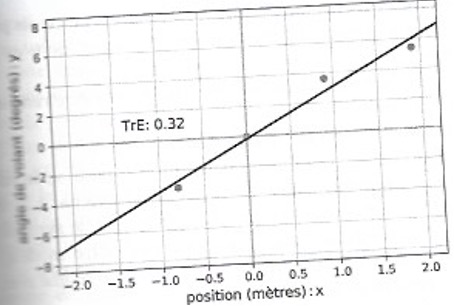
\includegraphics[width=0.7\textwidth]{images/graph2_yannLeCun.jpg} 
    \caption{Graphe page 88 du livre "Quand la machine apprend".}
\end{figure}
La pente passe par trois points sur quatre. Par conséquent, il faut trouver un compromis. On optera donc pour la solution où la droite passe au plus près des quatre points, comme modélisé précédemment. \\
%Conclusion Technologie voitures IOT
En somme, l’IoT révolutionne l’industrie automobile en offrant des véhicules plus sûrs, plus efficaces et mieux entretenus, tout en ouvrant la voie à de nouvelles innovations dans le domaine de la mobilité.\\
%conférence
La mobilité autonome vise à garantir un confort et une fluidité optimaux, ce qui nécessite un système de surveillance pour mesurer diverses variables. Cela se fait principalement par l'utilisation de capteurs embarqués.\\
L'orientation et la direction de la roue jouent un rôle crucial, tout comme la mesure des longitudes et l'utilisation d'unités de mesure inertielle (IMU). La mesure de la vitesse latérale, en revanche, requiert des capteurs très coûteux d'après la conférence\cite{ahmed_ali_synthese_2024} de Sofiane AHMED ALI.\\
Pour réduire le nombre de capteurs nécessaires et, par conséquent, les coûts de développement, on peut utiliser des observateurs\footnote{Observateur : Un outil mathématique ou algorithmique qui permet d’estimer des grandeurs internes d’un système (états) à partir de mesures disponibles et d’un modèle du système.} basés sur des modèles mathématiques pour déterminer les états du véhicule. Cette approche prometteuse présente toutefois des inconvénients, tels que la dynamique latérale du véhicule et les forces latérales agissant sur lui.
L'utilisation de capteurs visuels présente des défis supplémentaires. Ces capteurs peuvent allonger le processus de collecte de données et introduire des délais dans la transmission des images, ayant ainsi un impact majeur sur le système.


\newpage
\subsection{Les défis spécifiques liés à la sécurité des motos}

\subsubsection{Particularités des motos sur la route}
%•	Moins de visibilité et plus de vulnérabilité en cas d’accident.
%•	Dynamique de conduite différente des voitures (accélération rapide, inclinaison dans les virages).
Les motos présentent plusieurs particularités sur la route qui impactent leur sécurité et leur interaction avec les autres véhicules.
Une moto, c'est un véhicule de petite taille monté sur deux roues. Cela implique alors qu'elle est encore moins visible, surtout dans les angles morts d'un autre véhicule. Les motos sont agiles, possèdent une forte accélération et leur trajectoire est souvent imprévisible. Cela augmente le risque de collisions et les motos peuvent surprendre les autres usagers de la route. De plus sa configuration expose directement le conducteur deux-roues lors d'un accident par son manque de carrosserie. Les conditions météorologiques et la surface de la route jouent un rôle important dans l'adhérence des véhicules. Les conséquences matérielles et corporelles sont beaucoup plus importantes pour un deux-roues car la chute est inévitable.
La puissance de la machine demande beaucoup d'anticipation et une conduite plus exigeante face à tous les dangers.\\

Avec Mr Arioui, vice-président de l'innovation et des relations internationales, lors d'un échange, nous avons abordé l'importance du regard dans les trajectoires. En effet, le regard est essentiel pour anticiper les dangers et choisir la bonne trajectoire. De plus, tous les facteurs comme l'accélération, quand solliciter la moto influencent la trajectoire. 
La sécurité routière\cite{trajectoire_securite} met en avant cette technique nommée EDSR pour "Entrée, Découverte, Sollicitation de la moto, Reprise de stabilité" permet de prendre un virage en toute sécurité en augmentant le champ de vision afin d'anticiper les dangers. 
\begin{figure}[H]
    \centering
    \includegraphics[width=0.4\textwidth]{etat_art/images/trajectoire_securité.jpg} 
    \caption{Trajectoire de sécurité}
\end{figure}
Ci-dessous, l'importance de l'utilisation des trajectoires de sécurité. Cela permet d'anticiper les évènements qui arrivent en face de nous. Attention, c'est un exemple \textbf{parmi tant d'autres} (graviers, cyclistes, camions, bus, tracteur...).
\begin{figure}[H]
    \centering
    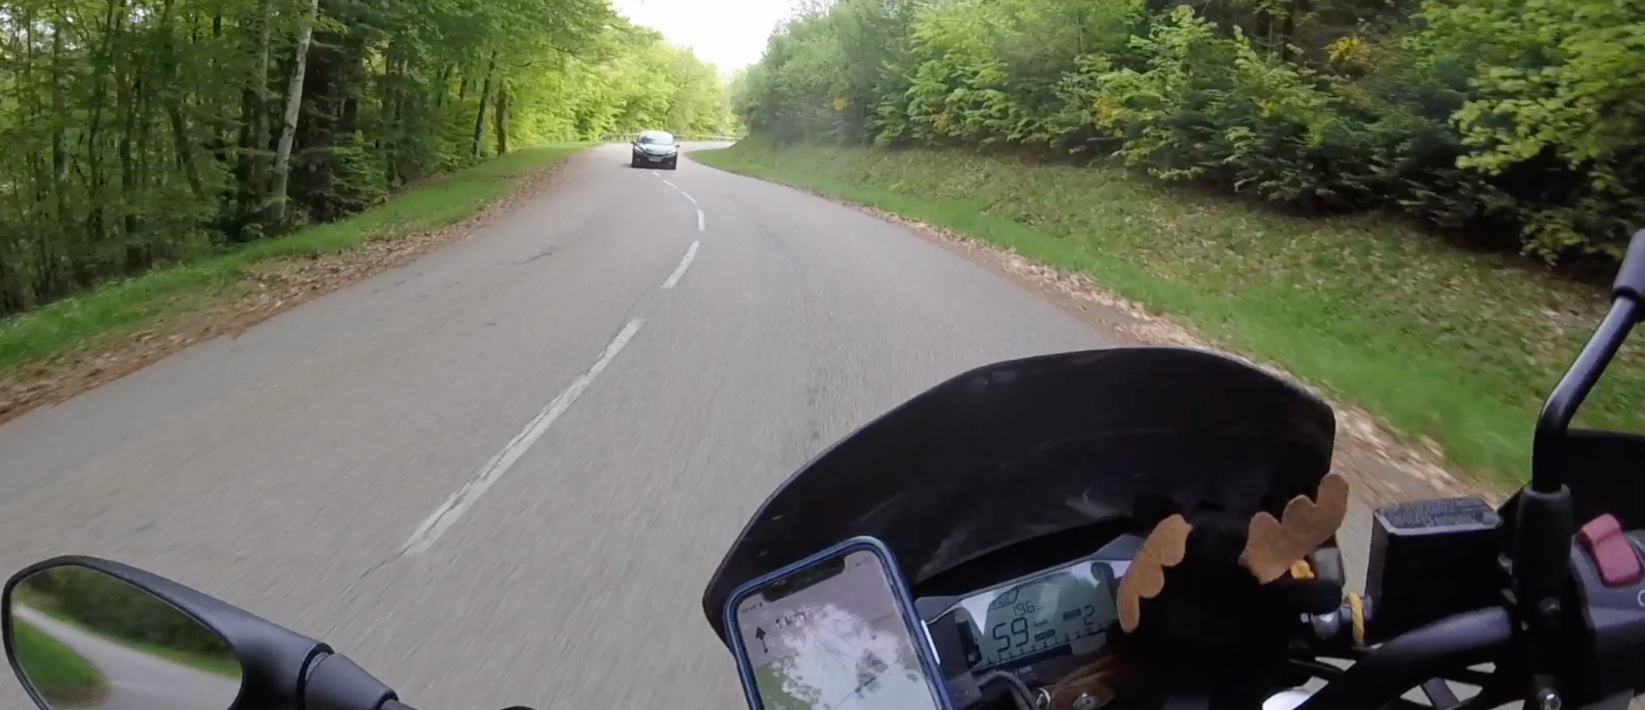
\includegraphics[width=0.6\textwidth]{etat_art/images/morvan.png} 
    \caption{Utilisation de la trajectoire de sécurité à moto}
\end{figure}
Pour mon retour d'expérience, le placement du regard est essentiel pour anticiper ce qu'il arrive en face. En se plaçant externe, cela permet donc d'agrandir le champ de vision et de pouvoir voir le véhicule qui arrive en face. En se plaçant interne, le champ de vision aurait été réduit et la collision entre les deux véhicules aurait été sûrement inévitable. De plus, la trajectoire de sécurité n'est pas toujours possible, il faut prendre en compte les autres facteurs : la vision (soleil), les véhicules arrivant en face, la qualité de la route...
Cette trajectoire est d'autant plus importante en montagne où les virages sont nombreux et les conditions de circulation peuvent être imprévisibles. La conduite en montagne nécessite une attention particulière, car les routes peuvent être étroites, sinueuses et parfois glissantes en raison des conditions météorologiques. Les motards doivent donc adapter leur conduite en conséquence, en réduisant leur vitesse et en restant vigilants face aux obstacles potentiels.
\begin{figure}[H]
    \centering
    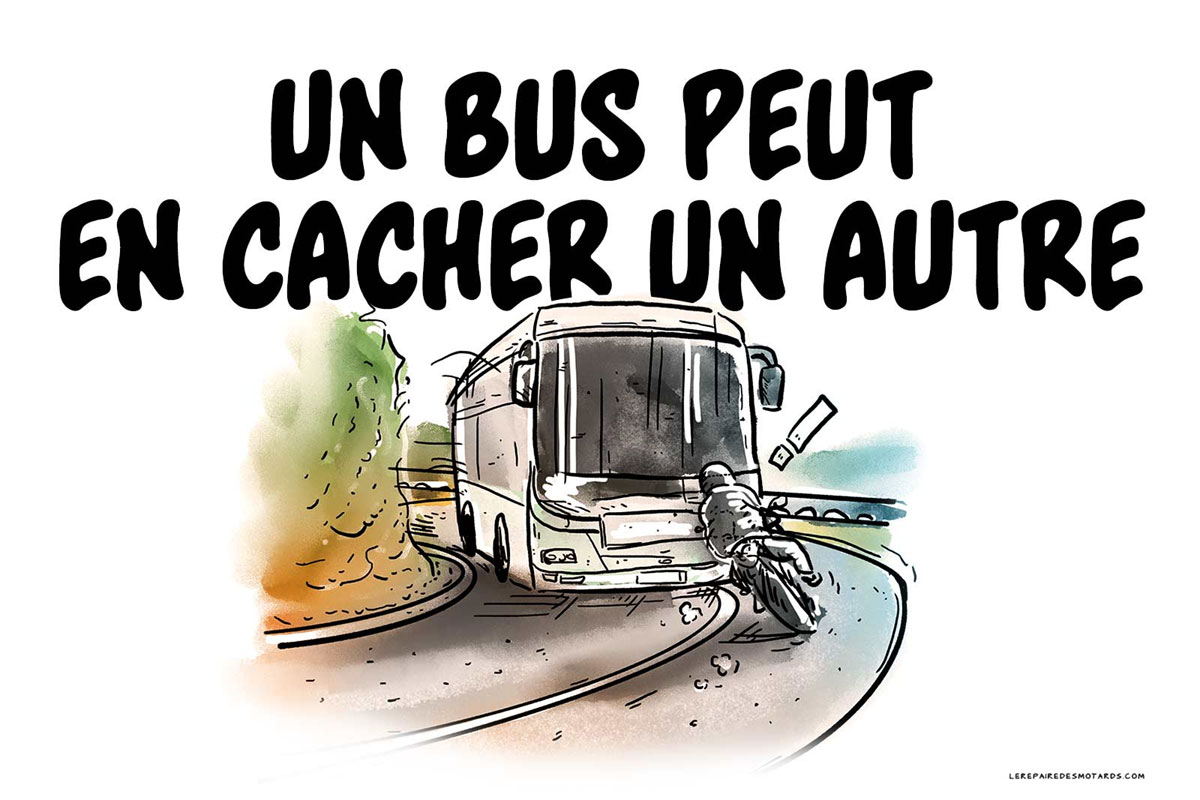
\includegraphics[width=0.6\textwidth]{etat_art/images/trajectoire-route-voie-bus-conduite_hd.jpg} 
    \caption{Illustration de la trajectoire de sécurité en montagne}
\end{figure}


\vspace{0.5cm} %conclusion
Ces particularités expliquent pourquoi la sécurité des motos sur la route est un enjeu majeur et nécessite des adaptations spécifiques dans les systèmes de détection et d’assistance à la conduite. 

\subsubsection{Les technologies IoT actuelles pour les motos}
%georide 
Aujourd'hui, de nouvelles marques, applications\cite{iot_accessoire_moto} apparaissent sur le marché de la moto. Cela créé également un écosystème permettant aux propriétaires de deux-roues de s'équiper à moindre frais (abonnement). Une des applications que nous pouvons exploiter sur le marché est Georide. Géoride une start-up française qui propose une solution de géolocalisation et de suivi des motos. Grâce à un boîtier connecté, les proches des motards peuvent suivre en temps réel leur trajet. Le boîtier est connecté à un réseau et il a la capacité à détecter une chute puis de contacter l'assistance. 
\begin{figure}[H]
    \centering
    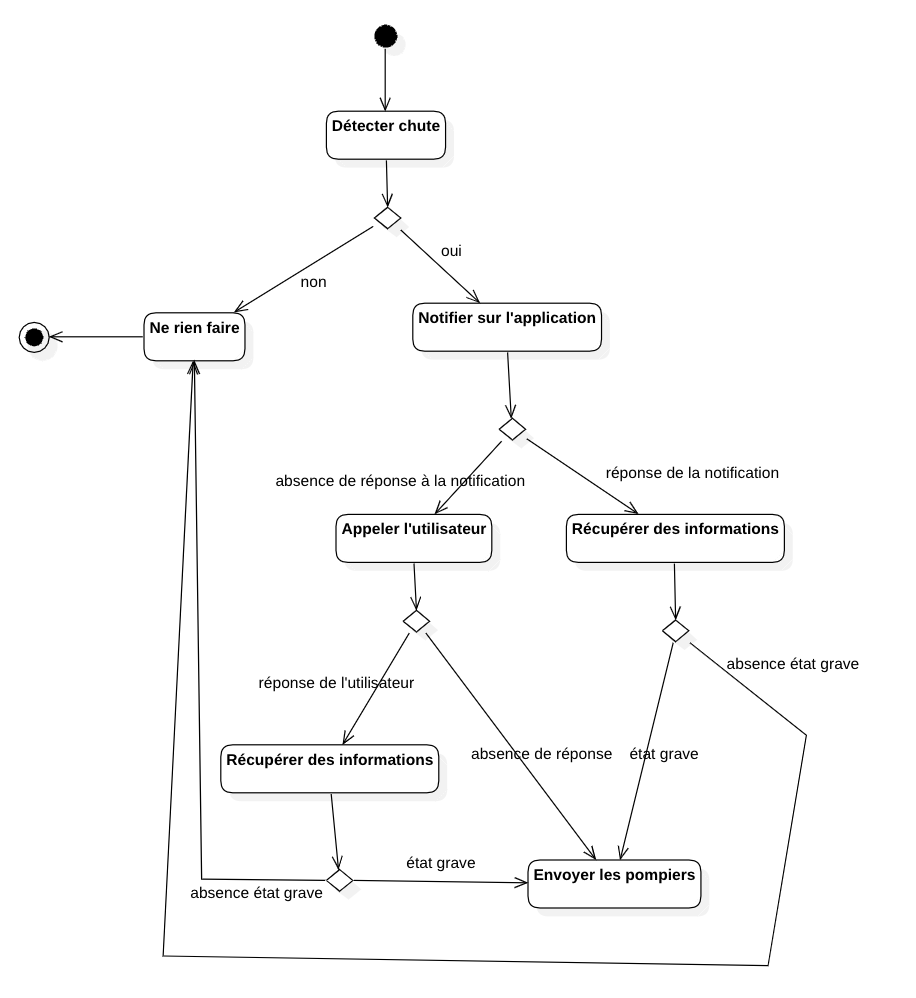
\includegraphics[width=0.8\textwidth]{images/diag_etat_georide.png} 
    \caption{Diagramme d'action du boîtier Géoride concernant la sécurité du motard}
\end{figure}
Ci-dessous, un témoignage d'un utilisateur de l'application Georide à la suite d'un accident à moto. Ce dernier souligne l'importance et le poids que peut avoir la technologie dans la sécurité des motards. Il évoque également la rapidité d'intervention des secours grâce à l'application, ce qui a permis de lui sauver la vie.
\begin{figure}[H]
    \centering
    \includegraphics[width=0.9\textwidth]{etat_art/images/témoignage géoride.png} 
    \caption{Témoignage d'un utilisateur de Georide sur le Discord de l'application réservé pour la communauté}
    \label{temoignage}
\end{figure}
Les dommages corporels sont très violents, même à faible vitesse. La rapidité est un facteur clé dans la survie d'un usager. L’application mobile fournit également des statistiques détaillées sur les performances du véhicule et des alertes en cas de vol ou de panne. Georide propose également des fonctionnalités de partage de trajet, des notifications sur l'entretien de la moto comme le graissage de chaine renforçant ainsi la sécurité et la convivialité de l’expérience de conduite.
\begin{figure}[H]
    \centering
    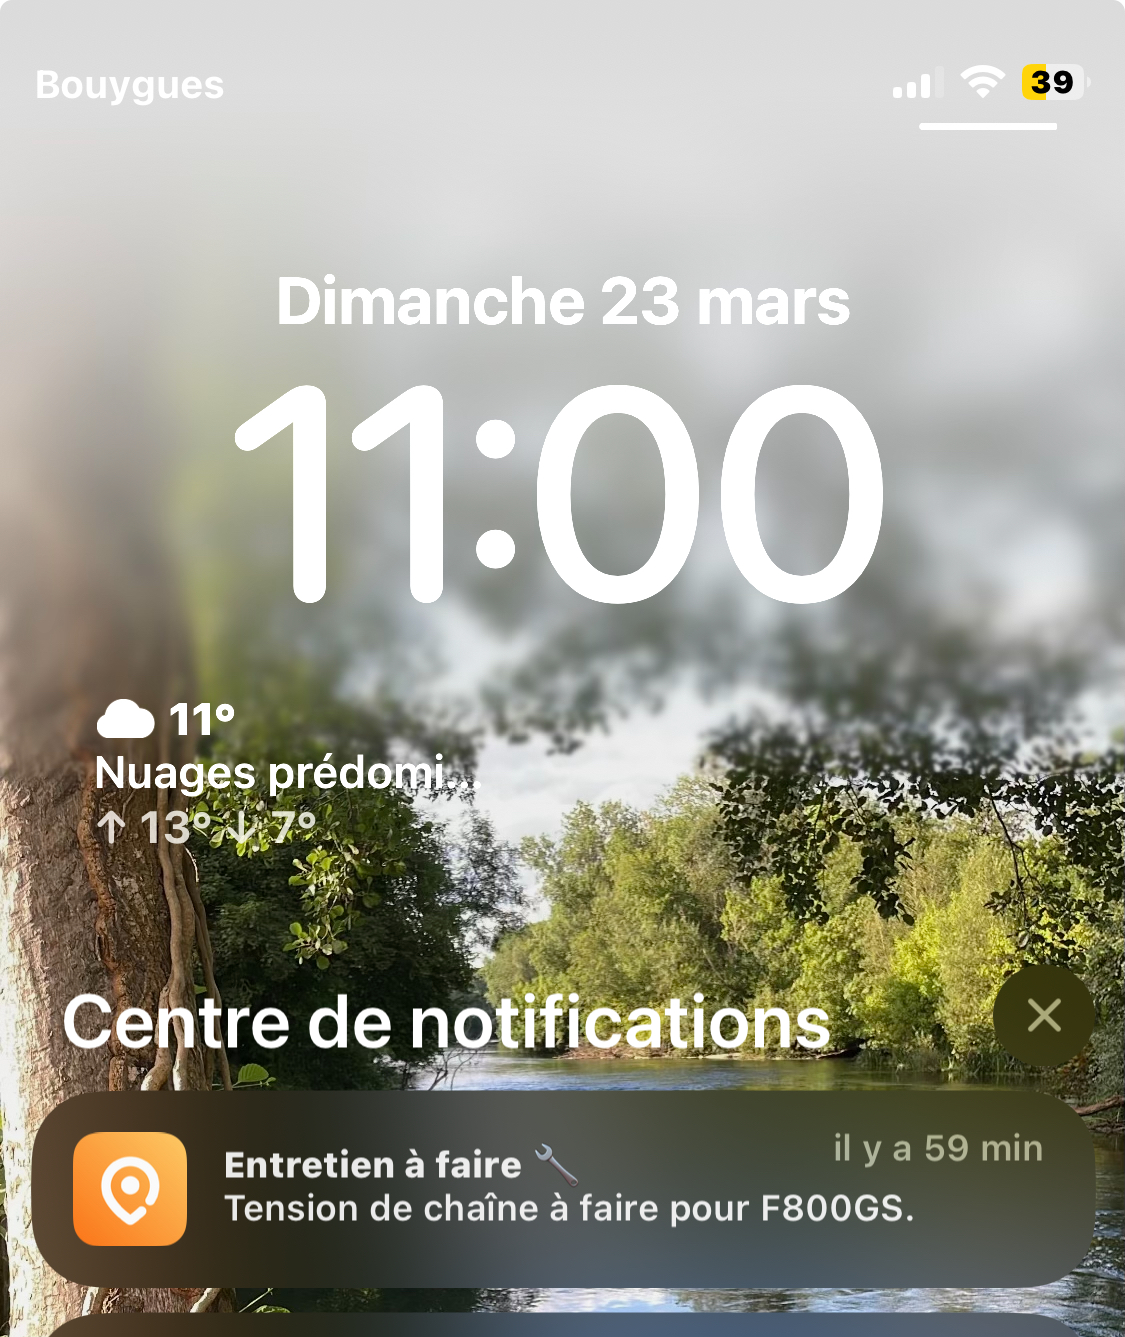
\includegraphics[width=0.5\textwidth]{images/notification_georide.jpg} 
    \caption{Exemple de notification de l'application Georide}
\end{figure}
Pour des motos qui n'ont pas l'option, il est possible d'y ajouter "Live Weel" qui permet de surveiller la pression et la température des pneus. Cela permet de réduire les risques de crevaison.
\vspace{0.5cm}

%Sena, cardo
Des dispositifs de communication sans fil sont également disponibles pour les motards. Des marques comme Sena et Cardo\cite{cardo} proposent des systèmes de communication mains libres qui permettent aux motards de rester connectés tout en conduisant. Ces appareils se fixent sur le casque et offrent des fonctionnalités telles que la communication intercom, la musique en streaming et les appels téléphoniques. Ils sont compatibles avec les smartphones et les systèmes de navigation, améliorant ainsi la sécurité et le confort des motards sur la route. Les dernières mise à jour concernent la détection de collision. Concernant le Packtalk Pro de chez Cardo, il est équipé de capteurs qui permettent de détecter une chute et d'envoyer un message d'urgence à un contact prédéfini.

%application
D'autres technologies sont plus accessibles comme celle qui est liée au téléphone. En effet, il existe des applications mobiles qui permettent de suivre son trajet, de partager sa position en temps réel et de recevoir des alertes en cas de danger. Ces applications sont souvent gratuites et faciles à utiliser et peuvent être prises en charge par les assurances: c'est le cas de Liberty Rider \cite{liberty_rider}. Cette application utilise les capteurs du smartphone pour détecter les chutes et envoyer automatiquement un message d'alerte à un contact d’urgence. Elle propose également des fonctionnalités de navigation, prévention des virages dangereux, de partage de trajet et de statistiques de conduite, améliorant ainsi la sécurité et la convivialité de l’expérience de conduite. D'autres applications comme Calimoto, 68 Degrés sont également disponibles et offrent des fonctionnalités similaires pour les motards.

%BMW
Pour des motos plus modernes, par exemple, BMW propose des motos connectées\cite{bmw_adas}. La moto est équipée de l’option « Connectivity » qui permet de connecter le smartphone à la moto via Bluetooth. L’écran TFT affiche les informations de navigation, les appels téléphoniques et la musique en streaming. La moto peut aussi être contrôlée via l’application mobile BMW Motorrad Connected, offrant des fonctionnalités de suivi, de maintenance et de partage de trajet. Ces technologies améliorent la sécurité et le confort des motards en leur permettant de rester connectés tout en conduisant.
%ADAS MOTO
Concernant les systèmes ADAS des motos\cite{moto_adas}, il y a des systèmes de freinage ABS,\footnote{Évite le blocage des roues.} de contrôle de traction et de suspension électronique qui sont de plus en plus courants sur les motos modernes. Ces technologies améliorent la stabilité, la maniabilité et la sécurité des motards en ajustant automatiquement les paramètres du véhicule en fonction des conditions de conduite. "De plus, tous les ADAS sur les voitures ne sont pas compatibles et ne seront pas d’une grande utilité sur les motos." d'après l'article de Moto-Net \cite{moto_adas}.
D'après une étude britannique, la technologie ADAS permet de réduire de 20 à 30\%\cite{moto_aras} les accidents de la route. Cependant, ces systèmes ne sont pas encore généralisés sur les motos et leur efficacité dépend de leur intégration et de leur compatibilité avec les spécificités de la conduite à deux-roues. La technologie équivalente à ADAS et ARAS\footnote{Advanced Rider Assistance System} est en cours de développement pour les motos et devrait être déployée dans les prochaines années.
Selon Geoff Liersch, président de la division Deux-roues et sports motorisés chez Bosch, "nous voulons améliorer la sécurité sans retirer le plaisir de la conduite"\cite{aras_bosh}.
Le système ARAS utilise des radars avant et arrière qui communiquent en permanence avec l’Unité de contrôle du moteur (ECU) et divers capteurs.

\begin{figure}[H]
    \centering
    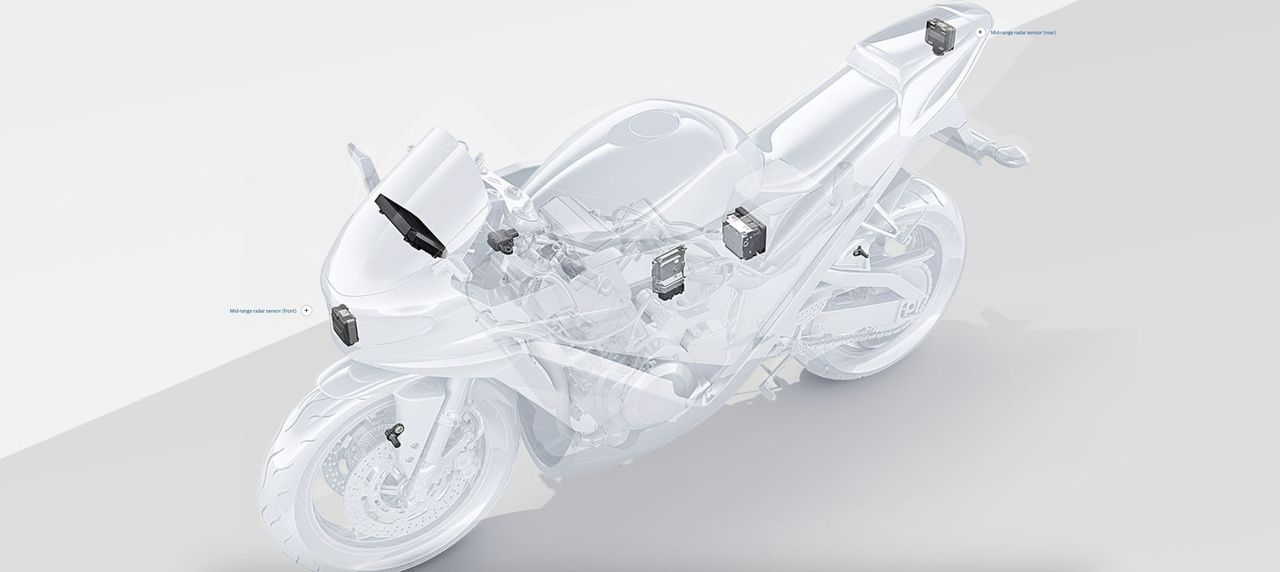
\includegraphics[width=0.7\textwidth]{images/aras_moto.jpeg} 
    \caption{Moto avec la technologie ARAS}
\end{figure}

%poursuivre avec la suite des tecnhologie
%radar adaptatif
Les radars adaptatifs, déjà utilisés dans l’automobile, font progressivement leur apparition sur les motos haut de gamme. Ce système utilise des capteurs radar pour :
\begin{itemize}
    \item Maintenir une distance de sécurité avec les véhicules qui précèdent.
    \item Avertir le conducteur en cas de risque de collision.
    \item Ajuste le freinage en fonction de l'inclinaison.
    \item Adapter automatiquement la vitesse et la distance de freinage.
    \item Détection d'angles morts.
\end{itemize}
Des constructeurs comme Ducati, BMW et KTM intègrent désormais ce type de radar sur certains modèles, améliorant ainsi l’expérience de conduite, notamment sur autoroute.

%perspectives
Plusieurs nouvelles aides et alertes sont en cours de développement pour les motos. Parmi elles, on retrouve :
\begin{itemize}
    \item Group Ride Assist : Aide à la conduite en groupe.
    \item Régulateur de vitesse adaptatif + Stop and Go : Maintien automatique de la distance de sécurité.
    \item Emergency Brake Assist: Illustré par la Figure~\ref{detecteuravant} est un freinage d’urgence en cas de risque de collision.
\end{itemize}

\begin{figure}[H]
    \centering
    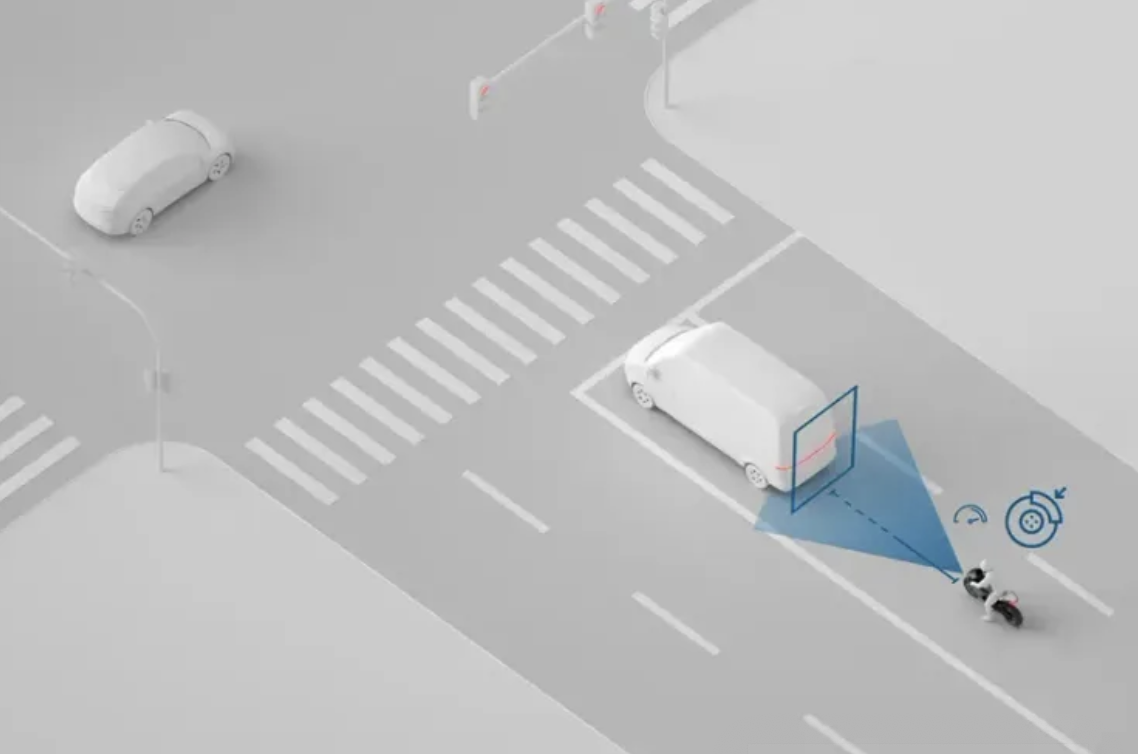
\includegraphics[width=0.7\textwidth]{images/ktm_detecteur_dev.png} 
    \caption{Moto avec la technologie ARAS pour un freinage d'urgence}
    \label{detecteuravant}
\end{figure}
- Rear Collision Warning: Illustré par la Figure~\ref{detecteurarriere}, il détecte si un véhicule s'approche trop près par l'arrière et active les feux de détresse en cas de risque de collision. 
\begin{figure}[H]
    \centering
    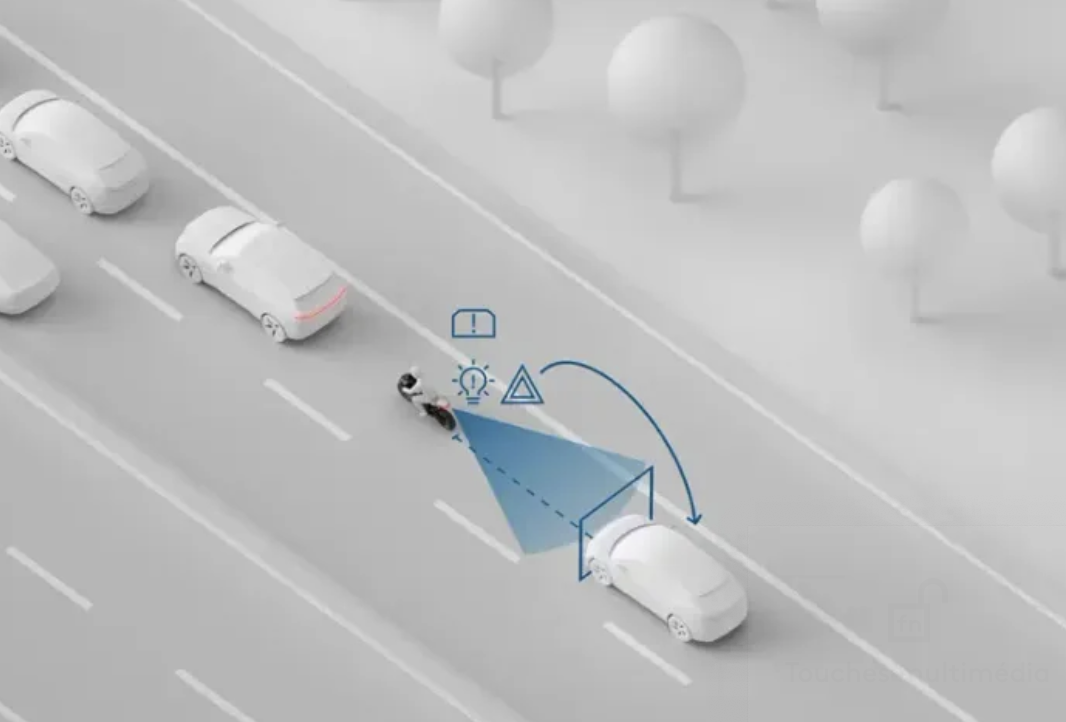
\includegraphics[width=0.7\textwidth]{images/ktm_detecteur.png} 
    \caption{Moto avec la technologie ARAS pour alerter en cas de collision arrière}
    \label{detecteurarriere}
\end{figure}

"L'objectif est d'avoir cette technologie pour une dizaine d'euros par moto. Cela pourrait réellement avoir un impact significatif sur la réduction des accidents." d'après Geoff Liersch.\\
%possibiliter de continuer les gaz lors de glissade
%abs spécifique moto

%moto autonomes bmw -> A REVOIR
Les motos autonomes sont en cours de développement, avec des prototypes. BMW Motorrad a présenté lors du Consumer Electronic Show 2019 (CES) à Las Vegas \cite{moto_autonome} un modèle de moto autonome capable de se déplacer sans pilote. Ce prototype, basé sur la BMW R 1200 GS, utilise des capteurs et des caméras pour détecter son environnement et naviguer en toute sécurité. Il est capable de démarrer, d’accélérer, de freiner et de tourner sans intervention humaine. 
Ce modèle intègre des technologies avancées telles que la conduite autonome, la connectivité et l’intelligence artificielle. Il est équipé de capteurs et de caméras pour détecter l’environnement et ajuster automatiquement la conduite en fonction des conditions de circulation. La moto est également dotée d’un système de stabilisation qui permet de maintenir l’équilibre même à l’arrêt, offrant ainsi une expérience de conduite plus sûre et plus confortable.

\begin{figure}[H]
    \centering
    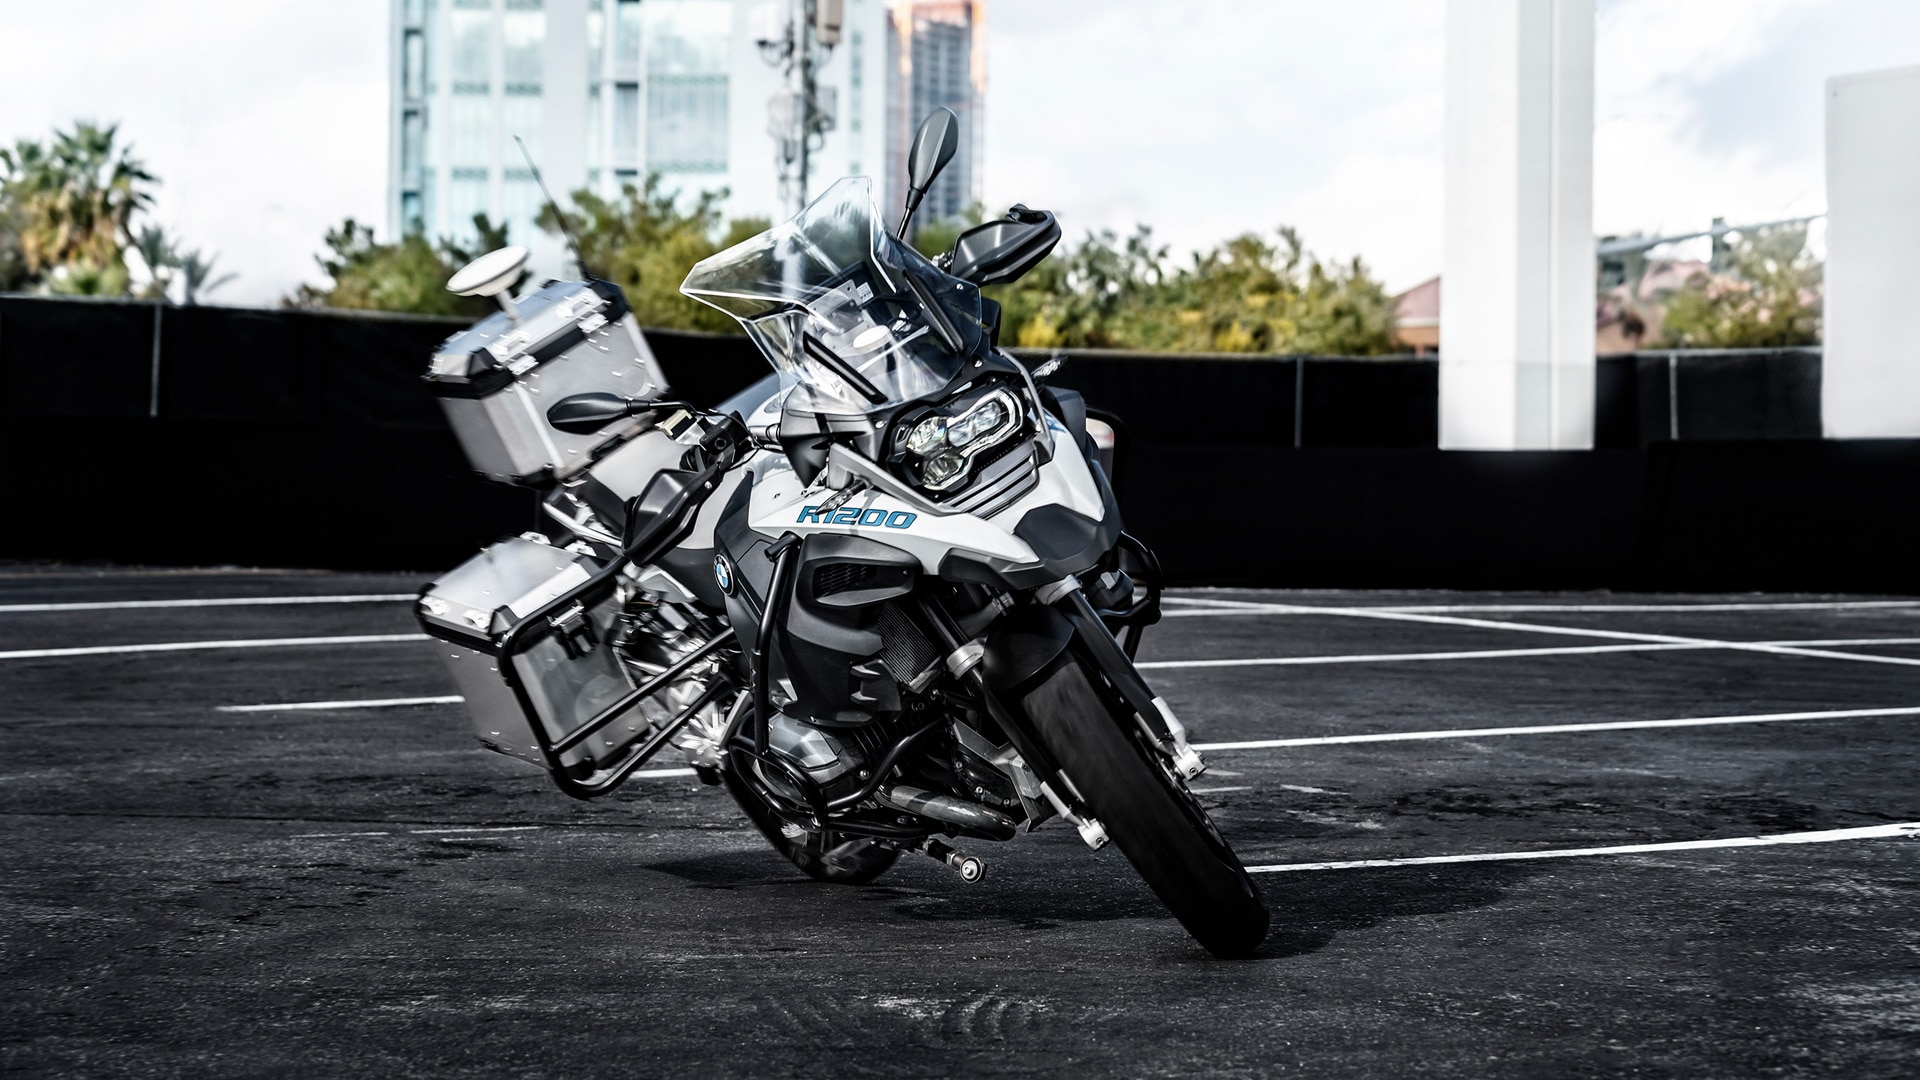
\includegraphics[width=0.7\textwidth]{etat_art/images/bmw.jpeg} 
    \caption{Moto R1300 GS autonome de BMW (2019)}
\end{figure}


%conclusion
L’intégration de ces technologies dans les motos modernes montre que l’innovation continue d’évoluer pour protéger les motards. Entre les radars adaptatifs, la gestion des gaz en cas de perte d’adhérence et l’ABS spécifique, ces avancées offrent une meilleure stabilité, un freinage plus efficace et une anticipation des dangers sur la route. L’avenir pourrait encore voir l’émergence de nouvelles solutions, comme la communication V2X (Véhicule à Tout) pour améliorer l’interaction entre motos, voitures et infrastructures routières.\\
Avec ces innovations, la moto de demain ne sera pas seulement plus rapide et plus performante, mais surtout plus sûre et plus intelligente. 

\subsubsection{L'exploitation des données pour les motos}
Avec l’essor des technologies embarquées et connectées, les motos modernes génèrent un volume croissant de données, dont l’analyse permet d’améliorer la sécurité, la maintenance et l’expérience de conduite.
Selon Bosch, les systèmes d’assistance basés sur le radar pourraient prévenir un accident de moto sur six \cite{aras_bosh_site_off}, en réagissant plus rapidement que le pilote dans des situations critiques. \\
Des projets comme Dymoa (Cerema) exploitent les données collectées lors des trajets réels pour mieux comprendre les risques propres aux deux-roues et adapter les politiques de sécurité routière.\\
Dans le cadre de mon alternance chez Kappa Santé, une entreprise spécialisée dans le traitement de données de santé sensibles, la protection des données personnelles est une priorité absolue. Des formations obligatoires sur le RGPD sont mises en place afin de sensibiliser les employés à ces enjeux. Cette exigence de rigueur en matière de sécurité m’a permis de mieux appréhender les enjeux liés à la collecte et à l’utilisation des données dans d’autres domaines, comme celui des motos connectées. Il est donc essentiel que les données générées par ces véhicules soient traitées avec le même niveau d’exigence : elles doivent être anonymisées, sécurisées et utilisées de manière responsable afin d’éviter toute fuite ou dérive dans leur exploitation.



\subsubsection{Limitations des technologies IoT actuelles pour les motos}
%•	Problèmes de détection par les capteurs des voitures autonomes.
%	•	Communication insuffisante entre motos et véhicules connectés.
%	•	Difficultés d’adaptation des infrastructures intelligentes aux besoins des motards.

%problème de détection
Le progrès côté deux-roues est très interessant et évolue.
La Verge TS Ultra est une moto électrique \cite{lenoir_cette_2024} haut de gamme intégrant des technologies avancées pour assurer une sécurité maximale à son pilote. Présentée lors du CES 2024, cette superbike est équipée du système Starmatter Vision, qui comprend six caméras et deux radars haute résolution, offrant une vision à 360 degrés de son environnement. Grâce à l’intelligence artificielle et au machine learning, la TS Ultra analyse en temps réel les risques potentiels et alerte le conducteur, notamment lors des changements de voie. Un écran agrandi sur le réservoir affiche des informations claires, comme la vue arrière lors de l’activation du clignotant. Côté performances, la moto à un moteur de plus de 204 chevaux, permettant une accélération de 0 à 100 km/h en 2,5 secondes. La Verge TS Ultra est disponible à partir de 54 880 euros.
Les technologies qu'embarquent les motos sont à la pointe mais coûtent très chères et ne sont pas encore accessibles à tous.\\
%yamaha
Yamaha, en collaboration avec Netflix, a donné vie à la moto futuriste Y/AI \cite{texier_quand_2024} , initialement imaginée dans la série animée “Tokyo Override”. Ce prototype a été exposé au Motor Expo 2024 en Thaïlande, illustrant la vision de Yamaha sur l’intégration de l’intelligence artificielle dans les motos de demain.\\

% moto electrique
Avec Mr Arioui, nous avons également abordé le sujet des motos électriques. Prenons l'exemple des voitures électriques.
D'après le site Ilek \cite{voiture_electrique}, le moteur électrique "Celui-ci est capable de fournir un couple instantané pour des accélérations fluides et dynamiques". Les voitures électriques ont les mêmes comportements que les motos électriques. Elles sont puissantes, réagissent instantanément. Leur couple\footnote{Plus un moteur est coupleux (qui possède du couple), plus sa capacité à tirer le poids total de la voiture ou d'une moto sera grande.} est élevé.
À la suite d’un échange avec Monsieur Arioui, il en ressort que les motos électriques ont un comportement totalement différent des motos thermiques. En effet, la puissance est instantanée et il n'y a pas de temps de latence entre l'accélération et la réaction de la moto. Cela demande une adaptation du motard. Lors d'une étude présentée lors de la 3ème réunion \cite{reunionProjet2025} à Nantes, il a été démontré que les usagers de motos électriques trouvent que les motos d'une cylindée équivalente à 125 cm3 sont seraient égales à celle d'un 600 cm3. La question soulevée est la suivante: "Faudrait-il un permis spécifique pour les motos électriques ?". Il est remonté également que la plupart des motards utilisent le mode éco pour limiter la puissance, le couple de la moto que pour limiter sa consommation.
De plus, le poids de la batterie est important et cela change totalement le comportement de la moto. Ce sont des points à prendre en considération pour la technologie de demain.
Une autre étude a été menée et présentée\cite{reunionProjet2025} sur le retour sensoriel de la vitesse des motards de la moto électrique. Cette expérience a été réalisé sur un simulateur. Il y a eu 21 participants. Les différentes expériences ont été réalisées avec ou sans vibration moteur, avec ou sans son... Une expérience avec l'absence visuelle montre une sur estimation de la vitesse. Par exemple, pour une vitesse de 50 km/h, les participants estiment la vitesse à environ plus de 65 km/h. Sans l'audition, la perception de la vitesse est faussée. Pour conclure cette étude, les étudiants ont noté que le visuel représente 41\%, le bruit du moteur représente 21\% enfin, la vibration, 14\%. Le défi ici est d'améliorer les zones d'attention. La décélération d'une moto thermique est de 3,8 km/h contre 5,5 km/h pour une moto thermique.
\vspace{0.5cm} %conclusion

\commentaire{la mentalité}
D'après une étude réalisée par « The American Automobile Association (AAA) »\cite{consumer_skepticim} en Janvier 2022, il y a 85\% de la population interrogée exprime leur inquiétude, leur peur face à la technologie des voitures autonomes. En effet, cette technologie doit encore faire ses preuves à la population bien que des résultats soient prometteurs.\\
De plus, les médias et les réseaux sociaux ont un impact important sur la perception de la technologie des voitures autonomes. Les accidents impliquant des voitures autonomes sont largement médiatisés et suscitent des débats sur la sécurité et la fiabilité de ces véhicules. Les constructeurs automobiles et les autorités doivent donc communiquer de manière transparente et pédagogique pour rassurer les usagers et favoriser l’adoption de ces technologies.\\
\vspace{0.5cm}

\commentaire{les accidents}
Les réseaux sociaux nous informent en temps réel des événements qui se déroulent dans notre pays ou à travers le monde. 
Récemment, j'ai lu un article (Annexe~\ref{articlevoiture}) daté du jeudi 1er août 2024, relatant un incident survenu en avril dernier. Il s'agit d'un motocycliste de 28 ans, percuté par une voiture en conduite autonome, une Tesla Model S de 2022. Selon les données recueillies, la voiture aurait effectué une embardée après avoir perçu un bruit, ce qui a conduit à la collision. Le fabricant rappelle que ces véhicules ne sont pas entièrement autonomes et que le conducteur doit toujours être prêt à reprendre le contrôle en cas de problème. Selon l'Administration de la sécurité routière des États-Unis, 75 autres accidents impliquant des voitures autonomes ont été recensés. 
La semaine dernière, Elon Musk, PDG de Tesla, a déclaré que d'ici la fin de l'année, les systèmes de "conduite autonome" devraient être capables de fonctionner sans la supervision constante de son conducteur.
\commentaire{limite juridiques}
\todo{limite juridique}
En cas d'accident, les lois concernant l'intégration d'aide à la conduite est complexe. Nous pouvons nous demander si les règles seront les mêmes que celles soumises aux voitures. Un décret de 2021 précise que si le conducteur respecte les conditions d’utilisation, il peut être dégagé de responsabilité pénale. Le constructeur devient alors pénalement responsable. Toutefois, le conducteur doit rester prêt à reprendre le contrôle lorsqu’il lui est demandé. Selon  Maître Sharon Bensemhoun-Gonzalez sur son site\cite{avocat}, les véhicules autonomes, aujourd’hui utilisés à divers niveaux d’autonomie (jusqu’au niveau 3 selon la norme SAE), soulèvent d’importantes questions en cas d’accident, notamment concernant l’attribution de la responsabilité entre conducteur, constructeur, ou fournisseur de logiciel. Le cadre juridique français reste flou en 2025, malgré les réflexions en cours au niveau européen. Chaque accident nécessite une analyse au cas par cas, souvent complexe pour les victimes. L’indemnisation reste un droit fondamental, notamment via la loi Badinter (1985), et ne peut être remise en question par l’innovation technique.\\
Maître Gonzalez distingue plusieurs situations possibles:
\begin{itemize}
    \item Erreur logicielle (par exemple Un freinage inapproprié par le système autonome)
    \item Défaillance d’un capteur (mauvaise perception de l’environnement)
    \item Inaction du conducteur obligé de reprendre la main 
\end{itemize}
Les responsables peuvent être :
\begin{itemize}
    \item Conducteur : responsabilité civile via l’assurance, même si son intervention n’était pas nécessaire en continu.
    \item Constructeur ou fournisseur : en cas de défaut technique ou vice, une responsabilité contractuelle ou liée à la responsabilité du produit peut être recherchée.
    \item Responsabilité pénale : possible en cas de négligence, désactivation de dispositifs de sécurité ou défaut d’entretien volontaire.
\end{itemize}
Enfin, la victime peut porter plainte ou bien établir un procès-verbal, réaliser des expertises (médicales, matérielle), demander une indemnisation et ou engager une action envers le constructeur. L'utilisation de boîtes noires sont utiles pour l’attribution des faits après accident. L'article\cite{tesla_condamnation} du 1er août 2025, un jury en Floride a condamné Tesla à ~243 M\$ dans un dossier d’accident mortel lié à « Autopilot ». Ce n’est pas du droit UE, mais c’est souvent cité en Europe car il illustre la façon dont des preuves logicielles et de conception sont discutées.\\
Même si l'évolution et le progrès de cette technologie impressionnent et présentent de bons résultats, la technologie montre de nombreuses limites et n'est pas encore au point.

\newpage
\subsection{Conclusion}
Bien que l’IoT offre de nombreuses opportunités pour améliorer la sécurité et l’efficacité des transports, il présente également des limites et des défis à relever. Ces limites peuvent lier à la technologie, la réglementation, la sécurité et à la confidentialité des données.\\
Chaque pays a sa propre réglementation et il est difficile de mettre en place une norme commune. Les constructeurs doivent donc s'adapter à chaque marché et respecter les lois en vigueur.\\
La sécurité des données est un enjeu majeur pour les véhicules connectés. Les données collectées par les capteurs et les systèmes embarqués peuvent être sensibles et nécessitent une protection adéquate contre les cyberattaques et les violations de la vie privée.\\
Enfin, l'interopérabilité entre les différents systèmes et véhicules est essentielle pour garantir une communication efficace et une coordination optimale entre les usagers de la route. Les technologies IoT offrent des solutions pour relever ces défis, mais leur mise en œuvre nécessite une collaboration étroite entre les constructeurs, les autorités et les utilisateurs pour garantir une mobilité plus sûre, plus intelligente et plus durable.
Pour conclure, chaque véhicule a des besoins spécifiques et le défi est de trouver des solutions adaptées à chaque type de véhicule. Les technologies IoT offrent des opportunités pour répondre à ces enjeux.\\
\newpage
\section{Mémoire}
\commentaire{Idées en cours ainsi que re formulation}


De nombreux systèmes IoT déjà présents sur les voitures trouvent également leur place sur les motos, tels que l’alerte d’angle mort, l’ABS, l’anti-patinage ou encore le contrôle de traction. Toutefois, malgré ces points communs, des différences significatives subsistent entre ces deux types de véhicules, notamment dans leur comportement et leurs contraintes spécifiques. Dans cette partie, je vais concentrer mon analyse sur l’évaluation de la route et sur les moyens d’optimiser la prise de trajectoire.


% faire des schémas avec les trajectoires pour souvelver les problèmes

\subsection{Pratique de la route - Analyse comparative des besoins de sécurité entre voitures et motos}

\commentaire{\\
Analyse des différences fondamentales : protection physique, stabilité, visibilité, comportements routiers.\\
	•	Quelles fonctionnalités IoT des voitures sont difficilement transférables ?\\
•	Quelles fonctionnalités sont transférables mais nécessitent adaptation ?\\
•	Mise en évidence des lacunes spécifiques aux motos.
}

J’ai eu l’occasion d’expérimenter la pratique du deux-roues sous différents angles :\
\begin{itemize}
    \item Les trajets du quotidien,
    \item Les balades entre ami(e)s,
    \item Les road trip de plus d'une dizaine de jours (environ 200 à 300 kms par jour), souvent en milieu montagneux.
\end{itemize}
Avec plus de 35 000 km parcourus en deux ans, voici les constats que j’ai pu faire autour de moi :
\begin{itemize}
  \item Les trajets du quotidien peuvent paraître anodins, mais c’est justement la routine qui les rend dangereux. En connaissant la route par cœur, on a tendance à relâcher sa vigilance, alors que les risques restent bien réels (état de la chaussée, comportement imprévisible des autres usagers, etc.).
  \item es balades entre ami(e)s apportent un vrai plaisir de conduite, mais l’effet de groupe peut parfois inciter à dépasser ses limites. On peut se retrouver à rouler à des vitesses inadaptées ou à prendre de mauvaises décisions sous l’influence de comportements plus audacieux. Le jugement individuel peut alors être altéré.
  \item 	Les road trips, quant à eux, demandent une grande endurance. La fatigue s’accumule rapidement, et avec elle, le temps de réaction s’allonge. Il est essentiel d’être pleinement en possession de ses capacités pour pouvoir réagir correctement en cas de situation imprévue.
\end{itemize}
Enfin, un point important : lorsque la chaussée est mouillée, la majorité des motards adoptent naturellement une conduite plus prudente, vitesse réduite, prise d’angle limitée, meilleure anticipation. Cela montre que la perception du risque influence fortement le comportement. %transition
Abordons maintenant une difficulté que beaucoup de deux-roues rencontres: les virages.

\subsubsection{Étude des virages}
%TRAJECTOIRES SECURITÉ
\commentaire{idée : montrer que c'est complexe}
Les illustrations ci-dessous représentent différentes trajectoires dites de sécurité. Ce sujet occupe une place centrale dans les campagnes de prévention menées par les acteurs de la sécurité routière. Il est régulièrement abordé par les forces de l’ordre, notamment les gendarmes spécialisés dans la sécurité des deux-roues motorisés, mais également par les formateurs, les auto-écoles et les usagers eux-mêmes.\\
En effet, la trajectoire de sécurité constitue une technique de conduite essentielle pour limiter les risques en virage, optimiser la visibilité et mieux anticiper les éventuels dangers. Elle permet au motard d’adopter une position plus stratégique sur la chaussée, en tenant compte à la fois du tracé de la route, de l’environnement, et de la circulation en sens inverse.\\
La sensibilisation à cette pratique est donc fortement encouragée, que ce soit lors des formations initiales, des stages post-permis ou à travers les communications des institutions publiques. Les illustrations présentées ici ont pour but de mieux comprendre ces trajectoires et de visualiser les choix possibles selon différents contextes routiers.
\begin{figure}[H]
    \centering
    \includegraphics[width=0.4\textwidth]{coeur_memoire/schéma/trajectoire_sécurité_1.png} 
    \caption{Trajectoire de sécurité utilisée sans obstacle}
\end{figure}
Adopter une trajectoire comme celle illustrée ci-dessus permet principalement d’optimiser la visibilité à l’entrée et dans le cœur du virage. En s’éloignant légèrement de l’intérieur de la courbe, le motard bénéficie d’un champ de vision plus large, ce qui lui permet d’anticiper plus facilement les éventuels obstacles, les changements d’adhérence ou la présence d’un autre usager.
Toutefois, cette trajectoire doit être adaptée dès lors qu’un autre véhicule circule en sens inverse. Dans ce cas, la priorité n’est plus uniquement la visibilité, mais également la sécurité du croisement. Il convient alors d’adopter une trajectoire dite de compromis ou "de sécurité", qui permet de conserver une marge de manœuvre tout en maintenant une distance suffisante avec le véhicule opposé.\\
La figure suivante illustre ainsi la trajectoire idéale à privilégier en présence d’un autre usager sur la route. Elle vise à garantir un passage fluide, sans empiétement sur la voie opposée, tout en maintenant une bonne stabilité du deux-roues dans la courbe. Ce type d’ajustement est essentiel pour réduire les risques de collision frontale, notamment dans les virages à visibilité réduite.
\begin{figure}[H]
    \centering
    \includegraphics[width=0.4\textwidth]{coeur_memoire/schéma/trajectoire_sécurité_4.png} 
    \caption{Trajectoire de sécurité utilisée avec un autre usager}
\end{figure}
Instinctivement, le motard va se rapprocher à l'extérieur du virage pour s'éloigner du danger représenté en bleu par la voiture.
Pour poursuivre cette démonstration, nous allons y ajouter d'autres dangers sur la route représentés par des objets en bleu rendant l'impossibilité de prendre une trajectoire "parfaite". Dans la vie courante, cela peut représenter des gravillons, un animal mort sur la route, des plaques d'égout, des nids de poule, des bandes d'étanchéité (mastics), etc. Ces éléments font perdre de suite l'adhérence des pneus et peuvent entraîner une chute. 
\begin{figure}[H]
    \centering
    \includegraphics[width=0.4\textwidth]{coeur_memoire/schéma/trajectoire_sécurité_2.png} 
    \caption{Autre configuration de la route avec plusieurs autres dangers}
\end{figure}
Ajoutons maintenant la trajectoire idéale à la situation permettant de garder l'adhérence des pneus:
\begin{figure}[H]
    \centering
    \includegraphics[width=0.4\textwidth]{coeur_memoire/schéma/trajectoire_sécurité_3.png} 
    \caption{Trajectoire de sécurité utilisée avec des dangers sur la route}
    \label{fig:trajectoire_securite_difficulte}
\end{figure}
Cette trajectoire améliore l’adhérence des pneus, mais elle présente un risque important en cas de danger venant en sens inverse. Si un véhicule surgit en face, le motard dispose de très peu de temps pour réagir ou se décaler, ce qui peut entraîner un accident. Il est donc essentiel d’adapter sa trajectoire en fonction de plusieurs éléments : l’état de la route, la visibilité et la présence d’autres usagers. La vitesse joue également un rôle déterminant : plus la moto roule vite, plus il devient difficile de corriger la trajectoire à temps. Voici ci-dessous plusieurs exemples de trajectoires, chacune présentant ses avantages et ses limites.
\begin{figure}[H]
  \centering
  \begin{subcaptionbox}{Trajectoire possible 1}[0.4\linewidth]
    {\includegraphics[width=\linewidth]{coeur_memoire/schéma/trajectoire_sécurité_7.png}}
  \end{subcaptionbox}
  \hfill
  \begin{subcaptionbox}{Trajectoire possible 2}[0.4\linewidth]
    {\includegraphics[width=\linewidth]{coeur_memoire/schéma/trajectoire_sécurité_6.png}}
  \end{subcaptionbox}
  
  \vspace{0.5cm}
  
  \begin{subcaptionbox}{Trajectoire possible 3}[0.4\linewidth]
    {\includegraphics[width=\linewidth]{coeur_memoire/schéma/trajectoire_sécurité_5.png}}

  \end{subcaptionbox}

  \caption{Autres exemples de trajectoires de sécurité}
\end{figure}

Annalysons et commentons ces trajectoires:\
\begin{itemize}
    \item Trajectoire 1 : C’est la plus sécurisante. Elle permet de s’éloigner efficacement du véhicule venant en sens inverse. Toutefois, si la vitesse est trop élevée, il sera difficile de revenir à l’intérieur du virage, comme le montre la trajectoire en vert.
    \item Trajectoire 2 : Elle est plus risquée, car elle place le motard plus près du danger potentiel. Même si la courbe semble fluide et permet une prise de virage à vitesse plus élevée, elle réduit la marge de manœuvre en cas d’imprévu.
    \item Trajectoire 3 : Elle représente un bon compromis, car elle maintient une certaine distance avec les véhicules en face. Cependant, rester trop proche du bas-côté peut s’avérer dangereux, notamment en cas d’obstacle imprévu (dégradation de la chaussée, présence d’un animal, etc.). La visibilité y est également plus restreinte, ce qui peut compromettre l’anticipation, l'analyse du virage.
\end{itemize}
Pour conclure sur ces schémas, il existe de nombreuses trajectoires possibles, mais peu sont réellement adaptées aux spécificités de la conduite moto. Certaines sont plus risquées que d’autres, et l’expérience du pilote joue un rôle clé dans le choix et la gestion de la trajectoire. Cela met en évidence à quel point cette phase de conduite est exigeante et complexe et combien de facteurs doivent être pris en compte pour envisager une assistance efficace.

%ETUDE SONDAGE
\subsubsection{Enquête auprès de motards - Recueil de ressenti}
J'ai réalisé une enquête dans différents groupes de motards sur les réseaux sociaux afin de récupérer leur ressenti. Il est très important pour comprendre la problématique de s'interessé à l'interessé. Cela m'a permis de mieux comprendre leurs besoins, leurs attendus afin d'avoir un oeil beaucoup plus objectif de ce que moi je peux vivre, ressentir. L'échantillon est composé d'une petite vingtaine de personnes avec 58,8 \% d'hommes contre 41,2 \% de femmes.
Voici les différents profils des participants :
\begin{figure}[H]
  \centering
  \begin{subcaptionbox}{Age des participants}[0.5\linewidth]
    {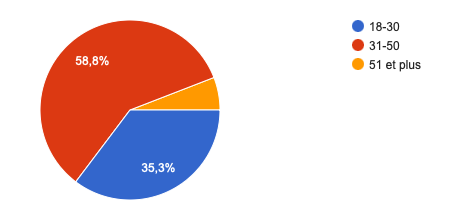
\includegraphics[width=\linewidth]{coeur_memoire/graphique/age.png}}
  \end{subcaptionbox}
  \hfill
  \begin{subcaptionbox}{Nombre d'années de permis}[0.5\linewidth]
    {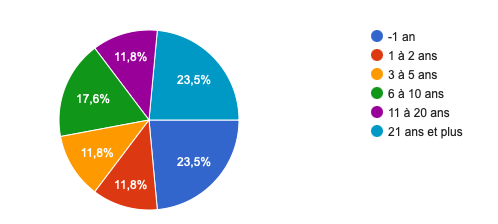
\includegraphics[width=\linewidth]{coeur_memoire/graphique/nb_annees_permis.png}}
  \end{subcaptionbox}

  \begin{subcaptionbox}{Nombre de kms à l'année}[0.5\linewidth]
    {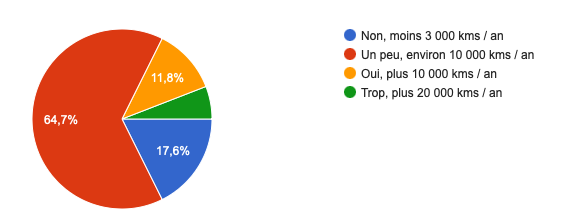
\includegraphics[width=\linewidth]{coeur_memoire/graphique/nb_km_an.png}}
  \end{subcaptionbox}
  \hfill
  \begin{subcaptionbox}{Utilisation de la moto}[0.5\linewidth]
    {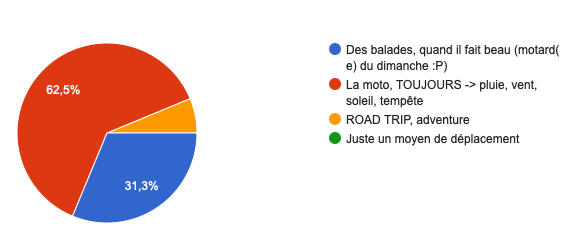
\includegraphics[width=\linewidth]{coeur_memoire/graphique/utilisation_moto.png}}
  \end{subcaptionbox}
  \caption{Profils des participants}
\end{figure}

Pour conclure, lors de cette enquête, il y a tous types de motards. Beaucoup roulent moins de 3 000 kms/an ce qui est très peu. C'est moins d'expérience sur la route.
Lors de mon enquête, la plupart des usagers possèdent des deux-roues roadster comme des 400 cc à 600 cc. On retrouve des Honda, Kawasaki, Aprillia, KTM et Yamaha. Ce sont des motos qui sont inférieures à 10 000 euros.
Pour les voyages, ou bien les voyages dans les Alpes, j'ai pu apercevoir une majorité de motards qui roulent en GS\footnote{Gelände/Straße : tout-terrain/route. C'est une moto conçue pour être à la fois confortable sur route et capable de rouler sur des chemins non gouderonnés. Premiers prix : 12 000 euros, haut de gamme : environ 30 000 euros.}. J'estime entre environ 50 et 70\% des motos rencontrées dans les Alpes (Suisse, Italie et France) sont des GS.\\
Voici quelques retours d'expérience des motards en situation d'urgence selon l'enquête :\\
• "Proche d'un rond-point, j'ai mal évalué la distance. Donc je suis arrivée trop vite, j'étais déjà dans l'insertion sur le rond-point et j'ai failli terminer dans un véhicule. Contrainte d'effectuer un freinage d'urgence et de me mettre le plus à l'extérieur pour éviter la catastrophe."\\
• "La voiture de La Poste stationnée en plein virage en sens inverse, empiétant sur ma voie. Sur une route à 50 km/h en agglomération. J'ai dû pratiquer l'évitement pour ne pas me prendre le véhicule."\\
• "Ma roue s’est coincée dans un rail de tram .. "\\
• "J'ai pris un trou (pas visible avant d'être dedans) sur une nationale, ce qui m'a fait guidonner, impossible à rattraper donc la moto a fini par se coucher et une belle glissade pour finir."\\
• "Évitement de personne qui tourne sans avoir mis de clignotant. Classique."
\vspace{0.5cm}

Pour la fin de l'étude, j'ai demandé aux participants quelles sont leurs attentes concernant les technologies IoT sur les motos. Certains ne souhaitent pas de technologie IoT, car ils estiment que cela peut nuire à la conduite et à la sensation de liberté. D'autres sont favorables à l'intégration de technologies IoT. Par exemple, un assistant virtuel qui indiquerait au pilote les dangers potentiels sur la route (chausée dégradée, virage dangereux, gravillon...). Les autres retours sont des technologies qui sont déjà présentes sur les motos du marché comme l'ABS, le contrôle de traction, l'anti-patinage, etc. Cependant, d'après certains motards, il faut mettre ces éléments de série et non en option comme l'appel d'urgence.
\vspace{0.5cm}

De plus, les réseaux sociaux relaient régulièrement des actualités concernant des accidents impliquant des deux-roues, illustrant la vulnérabilité des motards. Par exemple, un article (Voir ~\ref{articlemoto}) récent publié par Ouest-France rapporte qu'une jeune femme de 26 ans a perdu tragiquement la vie lors d'une leçon de moto-école dans l’Ain. L'accident s'est produit le samedi 2 août 2025 près de Châtillon-la-Palud. Alors qu'elle circulait sur une portion de route comportant plusieurs virages, elle a perdu le contrôle de son véhicule et percuté violemment une glissière de sécurité. La jeune femme n’a pas survécu à ses blessures. Aucun autre véhicule ne serait impliqué. Ce tragique événement rappelle une fois de plus l’importance d'améliorer constamment la sécurité des motards et l'importance de savoir bien aborder un virage.
\vspace{0.5cm}

Le véritable défi réside dans la capacité à adapter la trajectoire en temps réel, en fonction d’un ensemble de paramètres dynamiques et interdépendants. Cette adaptation ne dépend pas uniquement de la courbure de la route, mais également de nombreux vecteurs qui rendent la situation complexe à modéliser et à anticiper. Parmi ces vecteurs, on peut citer :\\
\begin{itemize}
\item La vitesse instantanée du véhicule, qui influence directement la trajectoire possible et le temps de réaction du conducteur ;
\item L’angle d’inclinaison de la moto, déterminant l’équilibre et l’adhérence lors de la prise de virage ;
\item L’état de la chaussée, incluant l’adhérence, les irrégularités, les débris ou l’humidité ;
\item Les conditions météorologiques, telles que la pluie, le vent, la chaleur ou le brouillard, qui impactent à la fois la visibilité et la tenue de route ;
\item La présence et le comportement des autres usagers, qu’il s’agisse de véhicules motorisés, de cyclistes ou de piétons ;
\item La géométrie de la route, incluant la largeur, le dénivelé, les virages successifs ou les intersections.
\end{itemize}
Dans ce contexte complexe, les technologies IoT (Internet of Things) peuvent jouer un rôle central. En fournissant des données en temps réel sur l’environnement routier, elles permettent de mieux analyser la situation et de faciliter la prise de décision. Par exemple, une communication entre véhicules pourrait alerter un motard d’un freinage brusque à venir, ou un capteur pourrait ajuster une recommandation de trajectoire en fonction de l’adhérence mesurée sur la route.\\
Il est important de rappeler que, malgré les apports technologiques, la trajectoire la plus appropriée reste celle dans laquelle le motard se sent en sécurité. Elle dépend fortement de son expérience, de ses réflexes, de sa confiance en lui et de sa connaissance de la route. Il n’existe donc pas une seule "bonne" trajectoire, mais une pluralité d’options, à ajuster en fonction du contexte, des données disponibles et des capacités du pilote.

%PLAISIR
\subsubsection{Défi passion}
\vspace{0.5cm}
Le plaisir de conduire une moto réside dans la sensation de liberté qu'elle procure. Cependant, cette liberté s'accompagne de responsabilités, notamment en matière de sécurité. Les technologies IoT peuvent contribuer à améliorer cette sécurité tout en préservant le plaisir de conduite. "Passionné auto moto depuis mon plus jeune âge, j'aime rouler souvent seul, mais j'aime me sentir libre et pouvoir aller où je veux et quand je veux, la moto, c'est indescriptible et c'est comme une drogue, mais c'est la passion." selon un retour de l'enquête.

\vspace{0.5cm}
Adapter l'IOT représente un défis car il faut prendre en compte de nombreux paramètres (environnement, comportement des usagers, etc.) et s'assurer que les solutions proposées sont adaptées à chaque situation.

\newpage
\subsection{ Étude critique des technologies IoT existantes (voitures vs motos)}
\commentaire{\\
avec un regard critique et des cas concrets.\\
Analyse de cas réels où les technologies IoT ont été adaptées à la moto (Airbags connectés, gilets intelligents, casques IoT, etc.).\\
  Freins techniques : taille réduite, alimentation électrique, exposition météo, vibrations, etc.\\
  lidar et radar ?\\
}

\subsubsection{Exemples d’IoT adaptés et développé pour la moto}
Plusieurs dispositifs connectés ont été développés spécifiquement pour les motards ces dernières années. Voici quelques exemples :
\begin{itemize}
  \item Airbags connectés (ex. : Dainese Smart Jacket, In\&motion avec Ixon): Ces gilets intelligents détectent les mouvements anormaux (chute, décélération brutale) via accéléromètres et gyroscopes, et déclenchent un coussin gonflable. L’algorithme est souvent connecté à une plateforme cloud qui analyse les données de milliers d’utilisateurs pour améliorer la détection.
  \item Casques connectés (ex. : CrossHelmet, Shoei IT-HT, Livall): Ils embarquent caméras arrière, GPS, commandes vocales, HUD\footnote{affichage tête haute} et parfois même des alertes de proximité de véhicules. Certaines marques permettent la communication entre motards via Bluetooth ou 4G.
  \item Systèmes d’aide à la navigation : Solutions telles que Calimoto, TomTom Ride... Offrent une navigation simplifiée pensée pour les deux-roues, avec une interface minimaliste et résistante aux intempéries.
\end{itemize}
Ces exemples illustrent que l’écosystème IoT appliqué à la moto progresse mais demeure nettement moins mature que celui dédié à l’automobile. Il serait donc pertinent de mesurer concrètement l’impact de ces technologies sur la sécurité, en s’appuyant sur des données chiffrées. Par exemple, quantifier la baisse du nombre de blessures graves grâce à l’utilisation d’airbags intelligents permettrait de dépasser le simple discours technologique pour appuyer les bénéfices réels.
La question de l’accessibilité reste également centrale. Le coût élevé de certains équipements comme un casque connecté pouvant varier entre 500 et 1500 euros peut représenter un frein pour de nombreux motards. De plus, la complexité liée à l’installation, à la configuration ou à la mise à jour de ces dispositifs peut décourager leur adoption à grande échelle.

\subsubsection{Les radars}
Aujourd'hui, de nombreuses motos sont équipées de technologies directement issues de l’industrie automobile, telles que l’ABS (système antiblocage des roues), la détection d’angle mort ou encore le régulateur de vitesse adaptatif. Ces dispositifs ont été progressivement adaptés pour répondre aux contraintes spécifiques des deux-roues, en tenant compte des enjeux liés à l'équilibre, à la maniabilité et à la sécurité du motard.
Après avoir expérimenté ces technologies, les retours des utilisateurs sont globalement très positifs. Ils mettent notamment en avant le gain en confort, particulièrement sur les longs trajets ou dans les conditions difficiles. Le régulateur adaptatif, par exemple, réduit significativement la fatigue en ajustant automatiquement la vitesse en fonction du véhicule qui précède. La détection d’angle mort accroît quant à elle la vigilance du conducteur, permettant une meilleure anticipation des dangers et réduisant ainsi les risques de collision.\\
L'intégration de ces technologies améliore non seulement l’expérience de conduite, mais contribue également de manière concrète à la sécurité routière. Moins sollicités sur des tâches répétitives, les motards conservent une meilleure concentration et sont donc moins exposés aux erreurs liées à la fatigue ou à l’inattention. Ces progrès montrent clairement l'intérêt de continuer à développer et à adapter des technologies automobiles avancées aux besoins spécifiques des utilisateurs de deux-roues motorisés.\\
%LIDAR
Les radars sont aujourd’hui intégrés aux modèles les plus récents de motos et remplissent efficacement leur fonction. Comme mentionné précédemment, la détection des éléments présents sur la route joue un rôle essentiel dans la sécurité du motard, tout comme les actions automatisées ou assistées qui en découlent. Ces technologies permettent notamment d’anticiper certains dangers, d’éviter des collisions ou de réguler la vitesse en fonction de l’environnement immédiat.\\
Cependant, les radars présentent certaines limites. Leur capacité à différencier les types d’objets ou à analyser finement l’environnement reste restreinte. C’est dans ce contexte que l’utilisation du LiDAR (Light Detection and Ranging) s’avère particulièrement intéressante. Cette technologie repose sur l’émission de faisceaux laser pour mesurer avec grande précision les distances et modéliser l’environnement en trois dimensions. Elle est très performante pour la cartographie 3D et la classification des objets, ce qui en fait un atout majeur dans les systèmes d’aide à la conduite avancés.\\

Néanmoins, le LiDAR n’est pas sans contraintes. Il reste très sensible aux conditions météorologiques défavorables telles que la pluie, le brouillard ou la neige, qui peuvent altérer la qualité des données recueillies. De plus, son intégration sur une moto pose plusieurs défis pratiques. La taille et le poids des capteurs peuvent affecter la maniabilité, l’esthétique et l’ergonomie de la moto. Sans compter le coût : en 2020, selon PW Consulting\cite{marche_capteur_lidar}, un capteur LiDAR compact se situait entre 3 000 et 10 000 euros — un prix difficilement envisageable pour la majorité des motards.\\

Heureusement, les coûts tendent à diminuer avec l’évolution du marché et la démocratisation de cette technologie. Aujourd’hui, il est possible de se procurer un capteur LiDAR pour un montant compris entre 500 et 2 000 euros, en fonction des gammes et des performances souhaitées. Cela ouvre de nouvelles perspectives pour une intégration progressive sur les deux-roues, à condition que les autres contraintes techniques soient également maîtrisées.\\

\vspace{0.5cm}
Les prototypes :\\
\begin{table}[ht]
\centering
\begin{tabular}{|l|c|}
  \hline
  Éléments & Prix \\
  \hline
  Capteurs LIDAR & 500 à 2 000 euros \\
  Traitement embarqués & 300 à 1 500 euros \\
  Interfaces et boîtier durci & 100 à 400 euros \\
  Intégration et calibration & 200 à 1 000 euros \\
  Total estimation & 1 100 à 5 900 euros \\
  \hline
\end{tabular}
\caption{Prix moyen estimé pour la technologie LIDAR sur moto (2025)}
\end{table}

Prenons les coûts moyens d'un deux roues :\\
\begin{table}[ht]
\centering
\begin{tabular}{|l|c|c|}
\hline
\textbf{Catégorie} & \textbf{Cylindrée} & \textbf{Prix moyen (TTC, €)} \\
\hline
Scooter & 50--125 cm³ & 2\,000 -- 4\,500 euros \\
Moto légère & 125 cm³ & 3\,500 -- 5\,000 euros \\
Moto moyenne cylindrée & 300--650 cm³ & 6\,000 -- 9\,000 euros \\
Moto grosse cylindrée & 700--1 000+ cm³ & 10\,000 -- 18\,000 euros \\
Moto sportive haut de gamme & 1 000+ cm³ & 18\,000 -- 30\,000 euros \\
Moto électrique & équiv. 50--125 cm³ & 4\,000 -- 12\,000 euros \\
\hline
\multicolumn{2}{|c|}{\textbf{Prix moyen toutes catégories}} & \textbf{7\,000 -- 9\,000 euros} \\
\hline
\end{tabular}
\caption{Prix moyen estimé des deux-roues neufs en 2025 (France/Europe) par The Market Reports}
\end{table}

\subsubsection{GPS}
Aujourd’hui, les systèmes GPS intégrés aux voitures ont atteint un haut niveau de maturité. Ils offrent une expérience fluide, fiable et parfaitement adaptée aux besoins de la conduite automobile. Les GPS modernes embarquent des composants hautement performants : un récepteur GNSS\footnote{Global Navigation Satellite System : capte les signaux émis par les satellites GPS, Galileo, GLONASS ou BeiDou pour calculer la position.}, des antennes optimisées, ainsi que des processeurs et chipsets de navigation capables d’interpréter rapidement les données satellites et d’exécuter des algorithmes de positionnement précis. L’ensemble est complété par des haut-parleurs intégrés, permettant de recevoir des instructions vocales sans quitter la route des yeux.
La situation est bien différente pour les motos. Ici, aucun habitacle ne protège contre la pluie, la poussière, les vibrations ou les chocs. Un GPS moto doit donc être conçu pour résister à ces contraintes. Cela implique l’utilisation d’un boîtier étanche et renforcé, conforme aux normes IP67/IP68\footnote{Les indices IP67 et IP68, définis par la norme IEC 60529, indiquent le niveau de protection d’un appareil contre la pénétration de poussière et d’eau.}, ainsi qu’un système de fixation robuste pour supporter les conditions de roulage. Les vibrations du moteur et de la route peuvent en effet détériorer des composants qui, dans un environnement automobile stable, ne subiraient aucun dommage.

\subsubsection{Contraintes techniques et comparaison voitures vs motos dans l’adoption des technologies IoT}

L’intégration de solutions IoT diffère fortement entre voitures et motos, en raison de contraintes physiques, énergétiques et environnementales propres à chaque type de véhicule. Le tableau \ref{tab:comparaison_iot_voiture_moto} présente une vue d’ensemble, suivie d’une analyse détaillée des points clés pour les deux-roues.

\begin{table}[H]
\centering
\caption{Comparaison des conditions d’intégration des technologies IoT entre voitures et motos}
\label{tab:comparaison_iot_voiture_moto}
\renewcommand{\arraystretch}{1.15}
\begin{tabular}{|p{3.2cm}|p{6.5cm}|p{6.5cm}|}
\hline
\textbf{Critère} & \textbf{Voiture} & \textbf{Moto} \\
\hline
\textbf{Espace disponible} &
Suffisant pour intégrer de nombreux composants électroniques (capteurs, unités de calcul, caméras, etc.) &
Très limité, surtout sur les modèles sportifs ou compacts ; intégration plus contraignante \\
\hline
\textbf{Alimentation électrique} &
Batterie de forte capacité alimentant de multiples systèmes &
Batterie réduite, imposant des dispositifs sobres en énergie \\
\hline
\textbf{Protection matérielle} &
Composants protégés par un habitacle fermé &
Composants exposés aux intempéries, à la poussière, aux vibrations et aux variations thermiques \\
\hline
\textbf{Sécurité passive} &
Ceintures, airbags frontaux et latéraux, zones de déformation &
Gilet airbag externe, casque et protections mécaniques personnelles \\
\hline
\textbf{Ergonomie d’affichage} &
Écrans tactiles, HUD, commandes vocales &
Affichage minimaliste via smartphone, casque connecté ou retour haptique/sonore \\
\hline
\textbf{Maturité des technologies IoT} &
Avancée (ADAS, V2X, LIDAR, conduite autonome partielle) &
Émergente (casques connectés, gilets intelligents, radars adaptatifs) \\
\hline
\end{tabular}
\end{table}

Pour les motos, la compacité des composants est un enjeu majeur : chaque capteur, antenne ou processeur doit être discret pour préserver l’esthétique et la maniabilité. La faible capacité électrique impose l’utilisation de modules économes en énergie. Les équipements doivent également résister à un environnement exigeant : exposition directe à la pluie, aux rayons UV, à la poussière et aux projections, avec un indice de protection d’au moins IP67 pour garantir la fiabilité.
Les vibrations et chocs, dus au moteur et à l’état de la route, nécessitent des fixations robustes et des matériaux résistants à l’usure. L’ergonomie est aussi déterminante : l’affichage des données, qu’il soit intégré au tableau de bord ou au casque, doit rester lisible et non distrayant. Ces contraintes cumulées expliquent que, malgré un fort potentiel en matière de sécurité et de confort, certaines innovations IoT restent encore peu démocratisées sur deux-roues.


\subsubsection{Pistes pour intégrer l’IoT dans les deux-roues}
Pour surmonter les limites actuelles, plusieurs pistes peuvent être envisagées :
Miniaturisation : développer des capteurs IoT plus petits et moins gourmands, spécifiques aux motos.
Énergie autonome : utiliser des solutions rechargeables ou solaires intégrées aux équipements (casque, gilet).
Normes de résistance : généraliser des composants certifiés IP67 ou supérieurs.
Interface modulaire : privilégier des alertes visuelles/sensorielles simples (LED, vibration, son), modulables par l’utilisateur.
Systèmes d’analyse distribués : partager les calculs entre un smartphone, un capteur embarqué et le cloud pour alléger la charge locale.
\vspace{0.5cm}

Pour conclure, la technologie LIDAR peut représenter à elle seule entre 12\% et 84\% du prix d'un deux-roues neuf mais le pourcentage reste moindre pour des voitures haut de gamme avoisinant les 50 000 euros. Cela reste très élevé pour un motard, surtout si l'on considère que la majorité des motards ne changent pas de moto tous les ans. De plus, il faut prendre en compte le coût de l'assurance, de l'entretien, du carburant, etc. Il est donc essentiel de trouver un équilibre entre sécurité et coût pour rendre ces technologies accessibles à tous les motards.

%Autre IOT
Concernant les autres technologies que peuvent proposer les autres marques, elles sont très pertinentes car elles sont destinées pour la sécurité des deux-roues et parfois élaborées par des motards eux-mêmes. Je pense à Géoride par exemple, qui est une application complète.\\
Ce qui peut être intéressant est d'avoir une interopérabilité entre les différents systèmes IoT. Prenons l'exemple de Géoride qui a un système de détection de chute, des motos peuvent l'avoir également ainsi que l'intercom Cardo. Cela permettrait d'éviter trois appels.

\subsection{ Proposition d’adaptation technologique}
\commentaire{	\\
•	Systèmes de communication V2X (Vehicle-to-Everything) pour motos : miniaturisation, portabilité, est ce que cela est possible ? les conditions.\\
	•	Capteurs embarqués sur la moto et sur le pilote (gilet, casque, smartphone).\\
	•	Intégration d’IA pour la détection du risque en temps réel : freinage d’urgence, angle d’inclinaison, anticipation de collision. => a voir\\
	•	Systèmes d’alerte connectés avec autres usagers (voitures, infrastructures).\\
	•	Possibilité d’un écosystème IoT dédié aux motos, interopérable avec celui des voitures. => à voir si ca existe déja\\
  • modélisation d'un tableau de bord connecté pour moto, avec des capteurs et des alertes en temps réel.\\
}

%PROPOSITION 1 : GPS MOTO 
\todo{parler également de l'accélération}

Pour pouvoir proposer de nouvelles fonctionnalités de prévention, il faut optimiser le tableau de bord. Il faut créer des logos communs à tous pour avoir le même langage. 

\todo{ajout d'un tableau de bord connecté avec des capteurs et des alertes en temps réel.}
L'idée serait d'intégrer dans les motos une puce GPS qui serait capable d'avertir en cas de virage dangeureux. L'alerte (sonore via un intercom et voyant au tableau de bord) serait envoyée via le tableau de bord connecté si la vitesse est supérieure à la vitesse recommandée. Cette vitesse sera calculée via la valeur de la courbure du virage. Des chercheurs Alex Liniger et Simon Hecker ont développé un prototype , Aegis Rider AG\cite{vitesse_virage_mcnews} permettant de prendre la meilleure trajectoire. Cependant, ce dernier ne prend pas en compte les autres facteurs de la route (autres usagers, état de la chaussée, etc.). Comme démontré ci-dessous, la trace bleu indiquant la trajectoire de sécurité et le compteur de vitesse masquent la qualité de la route par conséquent, le motard ne pourra pas anticiper les dangers de la route (gravillon, trous, ....). À l'heure d'aujourd'hui, cette solution reste extrêmement complexe. Ma solution permettra de fonctionner dans la pluspart des cas.

\begin{figure}[h]
    \centering
    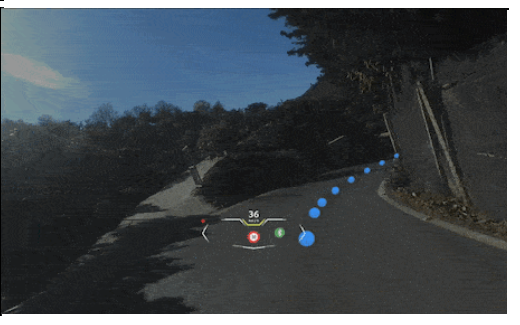
\includegraphics[width=0.7\textwidth]{coeur_memoire/images/aegis.png} 
    \caption{Prototype Aegis Rider AG pour la détection de virages dangereux.}
\end{figure}
Cette fonctionnalité est très interessante mais elle empêche une bonne visibilité de la surface de la route et elle peut fausser une prise de décision.
Comme illustré dans la Figure~\ref{fig:trajectoire_securite_difficulte}, le processus ne pourra pas adapter sur des virages dit "imparfaits".


\todo{voir pour faire une petite ligne de code ?}

\underline{Contexte:} En balade dans le 77, un motard roule sur une départementale. Dans cette situation, il est équipé d'un boitié GPS qui récupère ses coordonnées en temps réel. Il arrive dans une portion de virages limitée à 70 km/h nommée "Les 17 virages", près d'Arbonne-La-Forêt. Cette série de virages est dangeureuse car la route n'est pas bonne, n'est pas large et l'adhérence n'est pas optimale. De plus, il y a un virage dangereux à l'équerre qui surgit au milieu de cette série. La trajectoire de sécurité est fortement recommandé. Par expérience, avoisiner les 70 km/h est déjà bien au vue de la portion qui y est technique.

\begin{figure}[H]
    \centering
    \includegraphics[width=0.7\textwidth]{coeur_memoire/schéma/Capture d’écran 2025-07-24 à 15.45.48.png} 
    \caption{Point GPS des 17 virages.}
\end{figure}

\todo{photo des 17 virages}



Les coordnnées GPS sont : 48.385171, 2.563108.

\todo{mettre le diagramme}
Voici le diagramme d'action de cette fonctionnalité:\\

\begin{figure}[H]
    \centering
    \includegraphics[width=0.8\textwidth]{coeur_memoire/schéma/Capture d’écran 2025-07-24 à 17.48.10.png} 
    \caption{Diagramme d'action du Système de prévention de virages dangereux}
\end{figure}

Pour réaliser un bout de code sur cette fonctionnalité, j'ai décidé d'utiliser ces bibliothèques :\\
• osmnx\cite{osm_doc} : permet d’interroger OSM (OpenStreetMap) et de récupérer des graphes routiers.\\
•	geodesic (de geopy \cite{geopy}) : mesure la distance réelle (en mètres) entre 2 points GPS.\\

L'interêt de calculer la courbure de la courbe est de pouvoir anticiper le virage et par conséquent, adapter la vitesse pour optimiser l'adhérence, la trajectoire où l'on se sentira le plus en sécurité. \\
Le calcul de la courbure permettra d'identifier un virage s'il est dangereux à partir de données GPS cartographiques pour enfin adapter le comportement du système embarqué (alerte, adaptation de trajectoire, assistance..).
Donc la courbure mesure à quel point une route peut changer de direction sur une courte distance, ici, dans un virage.\\
Une route droite a une courbure environ égale à 0. Une route qui tourne fort (virage serré) a une courbure élevée.

\begin{table}[ht]
\centering
\begin{tabular}{|l|c|c|c|}
\hline
Route & Rayon du virage & Courbure (simplifiée) & Risque \\
\hline
ligne droite & infini & 0 & faible \\
Virage large autoroute & 500 m & Faible (0.01) & faible \\
Virage serré en montagne & 30 m & Forte (0.1–0.2) & Élevé \\
\hline
\end{tabular}
\caption{Exemple en pratique}
\end{table}

Un virage serré avec une courbure > 0.1 est souvent dangereux à +60 km/h, surtout à moto.
Plusieurs études indiquent que les rayons < 50 m sont classés comme virages dangereux pour les motos. À plus de 60 km/h, une moto doit pencher à plus de 35°à 40° dans le virage ce qui augmente énormément le risque de chute, surtout s’il y a du gravier, pluie, vent latéral…
L’estimation “courbure > 0.1 = danger > 60 km/h” est une règle empirique, basée sur des données de sécurité moto reonnues, des normes d'ingénierie routière et des approximations géométriques issues de GPS.


L'avantage d'avoir un calcul automatique et en amont, cela permet de prévenir avant même d'être dans le virage. Il peut remplacer un panneau quand celui-ci n'est pas visible. Elle ne remplace pas une analyse dynamique complète mais elle est suffisante pour alerter automatiquement le pilote ce qui est exactement l’objectif du système.



\begin{tcolorbox}[title=Calcul de la courbure]
Courbure mathématique\cite{formule_curvature} d’un virage:
\[
courbure\_virage = \kappa = \frac{1}{R}
\]
où R est le rayon du virage\\
Forme simplifiée de la courbure basée sur la déviation par rapport à une ligne droite.\\
a, b et c sont trois points dans la courbe.\\
\[
curvature = abs((a + b - c) / (a + b))
\]
a + b = distance réelle parcourue en suivant la route \\
c = distance directe entre le début et la fin (comme si on traçait une corde)
\end{tcolorbox}

\begin{figure}[H]
    \centering
    \includegraphics[width=0.7\textwidth]{coeur_memoire/schéma/Capture d’écran 2025-07-22 à 16.27.35.png} 
    \caption{Schéma présentant une moto avant un virage}
\end{figure}


\todo{illustration, développement}

\todo{Détailler le code}

\lstinputlisting[language=Python]{coeur_memoire/programme1.py}


\todo{résultat}
Suite de la mise en situation réelle. Les passages étudiés ont été réalisé bien avant l'expérience, par conséquent, il n'y a aucune notion de vitesse. Chaques passages ont été faits sur la capacité au moment t de l'usager. Voici un premier passage à 51 km/h.
\begin{figure}[H]
    \centering
    \includegraphics[width=0.6\textwidth]{coeur_memoire/images/Capture d’écran 2025-07-28 à 15.56.58.png} 
    \caption{Premier passage dans Les 17 virages}
\end{figure}

Résultat du premier passage avec le programme :
\begin{figure}[H]
    \centering
    \includegraphics[width=0.6\textwidth]{coeur_memoire/images/Capture d’écran 2025-07-28 à 16.23.05.png} 
    \caption{Premier passage dans Les 17 virages}
\end{figure}

Voici maintenant un second passage réalisé un peu plus vite.
\begin{figure}[H]
    \centering
    \includegraphics[width=0.6\textwidth]{coeur_memoire/images/Capture d’écran 2025-07-28 à 16.35.23.png} 
    \caption{Deuxième passage dans Les 17 virages}
\end{figure}


\begin{figure}[H]
    \centering
    \includegraphics[width=0.6\textwidth]{coeur_memoire/images/Capture d’écran 2025-07-24 à 16.20.18.png} 
    \caption{Deuxième passage dans Les 17 virages}
\end{figure}

Le deuxième passage est réalisé plus rapidemment (sans excès de vitesse), cependant, la vitesse est trop "rapide" et nécessite de meilleures capacités pour le passer. Il faut que le motard soit à un niveau bien intermédiaire. Comme l'objectif du programme est de faire de la prévention, j'ai décidé de baser sur un niveau de débutant. Pour conclure, il y a un message qui apparaît.

L'idée maintenant est de prévenir l'usager d'un logo universel. Évidemment, la disposition sera optimisée pour chaque écran. Nous pouvons également y ajouter un bip sonore, cela évitera de fixer en permanance le tableau de bord.
\begin{figure}[H]
    \centering
    \includegraphics[width=0.6\textwidth]{coeur_memoire/images/Capture d’écran 2025-07-25 à 14.42.42.png} 
    \caption{Génération d'un tableau de bord possible avec l'IA.}
\end{figure}



\newpage
\subsection{ Étude de faisabilité et limites}
\commentaire{\\
    •	Quels obstacles (coût, poids, énergie, connectivité, acceptabilité des motards) à l’implémentation ?\\
	•	Quelles pistes pour la recherche ou le développement industriel ?\\
	•	(une maquette fonctionnelle, un prototype conceptuel, ou même une étude de cas simulée)\\
  •	ouverture défi environnemental\\
  •	 protection des données sensibles (lien via kappa)        }


\subsubsection{Objectif de l'étude}
Cette étude vise à évaluer la faisabilité de la mise en œuvre d’un système d’assistance à la conduite basé sur l’analyse de la courbure de la route, dans le but de recommander une vitesse adaptée. Le système exploite des données géographiques pour déterminer la géométrie des segments routiers en fonction de la position d’un véhicule. Puis, il applique un modèle simple de calcul de courbure pour estimer la dangerosité d’un virage et proposer une vitesse conseillée. Ce chapitre examine les obstacles techniques, les contraintes d’implémentation réelle, ainsi que les perspectives de développement.

\subsubsection{Faisabilité technique}
Mon programme utilise des données routières open source via OpenStreetMap (OSM). Ces données sont accessibles et gratuites cependant, on apperçoit un manque de précision surtout en milieu rural. Certains segments peuvent manquer de points ou contenir des simplifications qui faussent l’évaluation de la courbure.
La méthode mise en œuvre repose sur le calcul géodésique entre trois points consécutifs, p1, p2 et p3 sur un segment de route à partir d'un point GPS, la position actuelle. Cela permet d’obtenir une estimation simple de la courbure.
Cependant, cette approche reste sensible à la densité des points sur les segments (peu de points donc cela implique une mauvaise précision).

\subsubsection{Faisabilité d’implémentation sur un véhicule réel}
Le monde du deux-roues posent certaines contraintes matérielles et logicielles :\\
\begin{tabular}{|l|l|}
\hline
\textbf{Élément} & \textbf{Détail} \\
\hline
Capteurs & Nécessité d’un GPS de bonne précision, module RTK pour éviter les erreurs de localisation.\\
Matériel embarqué & Un microcontrôleur\footnote{ (ex : Raspberry Pi, Arduino, ESP32) capable d’exécuter les traitements de calcul ou de les transmettre à une plateforme distante.}\\
Consommation & Ne doit pas être trop importante car ça reste un "petit véhicule" \\
Connectivité & Si les cartes ne sont pas embarquées, une connexion réseau est nécessaire, ce qui pose des limites en zone blanche.\\
\hline
\end{tabular}


Les limites actuellement restent les prix. En effet, ajouter des fonctionnalités de sécurité ayant des prix trop important baissent l'attractivité des motos. 

Comme il n’existe pas encore de produit commercial alliant GPS et l'alerte virage, on peut estimer sur la base des coûts de prototypes et de composants.\\

\begin{tabular}{|l|l|}
\hline
\textbf{Élément} & \textbf{Estimation de coût} \\
\hline
Capteur GPS + IMU (accéléro/magnétomètre)  & 50–200 € \\
Abonnement cartes HD (HERE, TomTom, etc.) &    10–30€ par mois   \\
Interface casque ou écran moto (HUD/haptique) au besoin & 100–300€ \\
\hline
\end{tabular}

\vspace{0.5cm}
Afin d'avoir un GPS précis et réactif. Il doit être accompané de la technologie IMU. IMU permet de compenser la latence et les imprécisions GPS en fournissant la vitesse angulaire (gyroscope) pour la courbure des virages, l'orientation (magnétomètre) et l'accélération linéaire (accéléromètre) pour les freinage. L'IMU peut fonctionner à 100-1000 Hz ce qui permet d'améliorer fortement le temps de réaction. Ces points sont crutiaux pour une fonctionnalité comme la notre, la prédiction d'abord de virages dangereux. La marge d'erreur n'est pas permise.

\vspace{0.5cm}
Voici un tableau comparatif:\\
\begin{tabular}{|c|c|c|}
\hline
\textbf{Propriétés} & \textbf{GPS} & \textbf{GPS + IMU} \\
\hline
Précision position & Environ 3 à 5 m & Bonne \\
Temps de réaction & Lent (de 0,5 à 1 seconde) & Rapide (<0,1 seconde)\\
Fiabilité en virage & Faible & Haute \\
Sensibilité du signal & Oui & Moins critique \\
\hline
\end{tabular}

\vspace{0.5cm}
L’acceptabilité d’un tel système dépend également du profil du conducteur. Un motard préfèrera un système non intrusif (affichage sur smartphone, retour haptique) et intuitif. Le système doit être discret afin de ne pas distraire l’attention ni le surcharger d’information. Un bip, un logo pourraient constituer une solution ergonomique.



\subsubsection{Prototype et simulation}

\subsubsection{Limites et contraintes}




\todo{mon programme}
Le programme fonctionne dans la pluspart des cas. Cependant, les données liant la limitation de vitesse n'est pas toujours récupérée. Par conséquent, par défaut la limitation de vitesse est 80 km/h. Sur les portions d'autoroute, la limitation est de 130 km/h et la courbure a une valeur quasiment nulle. Prenons un cas où la limitation est 110 km/h, il faut que la courbure soit suffisamment élevée pour ne pas pouvoir prendre un virage à plus de 80 km/h. C'est un risque accepté et réfléchi pour ce programme.
Concernant la fonctionnalité, certains motards peuvent percevoir cette aide comme trop "prévoyante". En effet, plus un motard roule et plus il acquière de l'expérience, sous condition qu'il varie les types de trajet. Il peut donc se dire que l'alerte arrive trop tôt. On peut donc prendre en concidération une variable de niveau qui propose un déclanchement de l'alerte selon une certaine vitesse. L'accélération est un facteur que l'on peut également prendre en compte. À un niveau de jet avant un virage peut suffir pour avertir d'un danger.
De plus, on constate que le programme (Figure~\ref{fig:cartepoints}) se base uniquement sur l’instant présent, sans prendre en compte la trajectoire ou la direction future du motard.



\todo{développer la partie loi + internationnal}
L'utilisation du GPS est très réglementé, surtout dans les pays. Le défi ici c'est de se demander comment peut-on développer des technologies, des innovations qui respectent les règles, la confidentialité des usagers des pays concernés.\\

Par exemple :\\
La Chine autorise le GPS mais avec un accès limité à certains services cartographiques. Dans plusieurs pays comme l'Autriche, l'Allemagne n'autorise pas les GPS avec les avertisseurs ou détecteurs de radar. Au Japon, le GPS est autorisé mais certains appareils RF\footnote{Radio Fréquence : Ce sont des dispositifs qui émettent et recçoivent des ondes radio pour communiquer entre 3 kHz et 300 GHz.} sont interdits.


\todo{défi affichage en respectant la loi}
L'utilisation du GPS est autorisé quand celui-ci ne gêne ni la visibilité, ni la conduite d'après Code de la route français – Art. R412-6\cite{loi_code_de_la_route}.

\todo{rgpd}
Le GPS va recueillir des données, suivre l'usager. Pour approfondir et améliorer le système, des données seront collectées par conséquent, le consentement explicite du motard est nécessaire. Il faut également ajouter une déclaration ou une politique de confidentialité claire.
\todo{kappa métier séparer}

\todo{vitesse donc puissance max et reformuler}
Comme certaines motos sont "rapides", il ne faut pas oublier que les motos sont des véhicules qui roulent beaucoup plus vite (accélération, vitesse). Cela impose donc d'avoir du matériel de qualité permettant d'avoir un temps de réactivité et une puissance de calcul qui répondent à cette caractéristique. De plus, comme la sécurité est un enjeu primordial, les points GPS ne peuvent pas forcément être précis, c'est un cas qu'il faut gérer.

\todo{proposition rédaction rgpd}
Il faudra collecter que les données nécessaires position, vitesse, horodatage. Les données doivent être stockées dans une base de données sécurisées et chifrées.

\todo{choix, marque du produit}
Voici des propositions de composants que nous pouvons utiliser : 	\\
•	u-blox NEO-M8N : excellent rapport qualité/prix, ~40 € \\
•	u-blox ZED-F9P : haute précision RTK, mais cher (~200–250 €) \\
•	SparkFun GPS + IMU : combine ZED-F9P + BNO080 (IMU)\\






\newpage
\subsection{Apport personnel et positionnement}
\commentaire{Une prise de conscience collective}
La sécurité n’a pas de prix. C’est un principe fondamental qui devrait guider tout développement technologique appliqué aux transports. Si les voitures bénéficient depuis plusieurs années de dispositifs de sécurité avancés comme de l’ABS à l’assistance au maintien de voie, les deux-roues motorisés restent, en comparaison, bien plus vulnérables. Et pourtant, la pratique du deux-roues s’étend, elle attire un public passionné, exigeant, conscient des risques mais aussi demandeur d’innovation.\\
Aujourd’hui, la réflexion autour de la sécurité moto ne doit pas uniquement se limiter à des équipements de protection ou à des comportements individuels. Elle doit intégrer une vision systémique, dans laquelle l’environnement, les infrastructures, la technologie embarquée et l’intelligence collective des usagers jouent un rôle complémentaire.\\
\commentaire{Une technologie encore en transition}
De nombreux projets technologiques sont en cours. L’ABS est désormais obligatoire sur les motos de plus de 125 cm³ et certaines marques comme BMW, Honda ou Yamaha explorent déjà des systèmes d’assistance avancés : 
\begin{itemize}
	\item Détection d’angle mort,
	\item Alertes de collision,
	\item Freinage adaptatif.
	\item ...
\end{itemize}
Mais ces dispositifs restent encore peu répandus, coûteux ou en phase de test. La moto, par sa nature même :
\begin{itemize}
	\item Équilibre dynamique,
	\item Surface réduite,
	\item Exposition aux éléments.
\end{itemize}
Représente un défi technique beaucoup plus complexe que la voiture. Tous les paramètres doivent être pensés avec précision comme l'inclinaison, l'adhérence, la vision périphérique, le comportement du pilote, l'état de la chaussée, etc.\\
Il est difficile de modéliser l’ensemble de ces facteurs dans un algorithme simple. Certaines situations et certains facteurs restent imprévisibles. Et parfois, aucune formule ne suffit à expliquer un comportement ou une prise de décision sur la route. Certaines actions sont sur l'instinct. D’où l’importance de ne pas tout miser sur l’automatisation mais de construire des outils d’assistance intelligents conçus comme un appui à la prise de décision, et non comme un remplacement du jugement du pilote. C'est pour cela qu'évoluer une trajectoire parfaite n'est pas facile.\\
\commentaire{Une évolution des mentalités}
Heureusement, les mentalités évoluent. Le motard d’aujourd’hui n’est plus seulement un amateur de sensations fortes, c’est aussi un usager averti, souvent bien informé, conscient des limites de sa machine et soucieux de sa sécurité. À condition qu’elles soient bien expliquées, justifiées et qu’elles apportent une réelle valeur ajoutée à l’expérience de conduite, les innovations technologiques ont de fortes chances d’être acceptées.
Il ne s’agit donc pas simplement de créer une technologie nouvelle mais de proposer des solutions pertinentes, pensées avec les utilisateurs, testées dans des conditions réelles, et intégrées dans un écosystème cohérent. La sensibilisation et l’éducation auront également un rôle clé à jouer pour accompagner cette transition. Nous pourrons nous référer aux moniteurs écoles par exemple, aux constructeurs...
De plus, des lois doivent être plus claires et mieux mises à disposition des concernés afin de ne pas être surpris.\\
\commentaire{Une vision d’ensemble : combler le fossé}
À terme, ce travail s’inscrit dans une dynamique plus large : celle de combler le fossé technologique entre la sécurité automobile et la sécurité des deux-roues motorisés. Ce n’est qu’en intégrant les spécificités de la moto dans les démarches de conception, de régulation et d’innovation que l’on pourra répondre aux besoins réels des motards. Une mobilité durable, inclusive et sûre ne pourra exister sans penser à ceux qui, chaque jour, prennent la route sans carrosserie pour les protéger.

\newpage
\section{Conclusion}


\subsection{Conclusion mémoire}
\todo{reformuler}
Mes recherches n'étaient pas évidentes, mon univers de travail n'est pas orienté sur les véhicules, l'automatisation... J'ai eu la chance d'avoir eu l'opportunité de travailler sur un sujet qui me tenait à coeur. Lors de mon travail, j'ai pu faire de superbes rencontres et assiter à des travaux uniques. Cela m'a permis de découvrir cette univers de la moto sous un oeil scientifique. Découvrir également les contraintes. Même s'il n'y avait pas beaucoup de point commun avec mes missions en alternance, on peut retrouver les mêmes défis comme la protection des données.
Développer de la technologie pour la sécurité, surtout pour les deux roues représente un reel défis et aujourd’hui, beaucoup d'ombre reste à ce sujet.



\subsection{Conclusion année d'alternance}
\todo{reformuler}
Cette année et ce travail concluent trois années à Kappa Santé où j'ai beaucoup appris tant au niveau de la mission d'un développeur que du relationship. 
Je m'oriente maintenant vers de nouveaux horizons.

 
\newpage
\printbibliography
\addcontentsline{toc}{section}{Références}

\newpage
\appendix
\section*{Annexes}
\addcontentsline{toc}{section}{Annexes} 
\section{Échange avec Hichem ARIOUI}
Voici l'échange transcrit que j'ai eu avec M. Hichem ARIOUI sur les deux-roues motorisés le 9 mai 2025 à l'Université d'Évry (Bâtiment Île de France). \\
Hichem ARIOUI : Donc tu fais quel parcours exactement? \\
Shana : En moto, moi, je fais tout. Que ce soit de la route, l'autoroute, des chemins de campagne.\\
Hichem ARIOUI : D'accord. \\
Shana: Et j'aimerais me mettre aussi à l'off road. C'est un peu... Ce n'est pas vraiment du cross, mais c'est autre chose. \\
Hichem ARIOUI : Ok, très bien. Moi, [...]je fais de la moto. Je ne le fais pas ici en France, je le fais en Indonésie. Mais c'est plutôt des scooters. Ok. Des X-max, des T-max. Voilà, tout simplement. Mais je connais, c'est un domaine sur lequel je travaille depuis 2000... 2005, 2004, quelque chose comme ça. \\
Shana: D'accord. Oui, j'ai vu un peu ce que vous travaillez. Là, c'est en ce moment sur les motos électriques, pardon? Là, en ce moment, oui, \\
Hichem ARIOUI: c'est des motos électriques parce que c'est une difficulté un peu étrange, parce que la façon dont on accélère et on freine, le couple, il est instantané. \\
Shana: Oui, on le voit avec les Tesla, par exemple. \\
Hichem ARIOUI: Exactement. Mais ouais. Et pour freiner, accélérer, parfois, ça t'emmène vraiment vers des situations de dérapage que tu ne peux pas contrôler forcément. \\
Shana: Malgré l'ABS et autres? \\
Hichem ARIOUI: Ben oui. L'ABS, généralement, quand on peut le débloquer, les motards le débloquent. Ce qu'ils veulent pas-- ce qu'ils cherchent, les motards, pas les novices. Je parle des expérimentés. C'est plutôt la liberté de faire ce que je veux. Donc, tu n'es pas le TCS, le MCS, le machin. Ça, ils désactivent. Ils n'aiment pas. \\
Shana : Moi, j'ai la chance, c'est que j'ai une moto vraiment récente qui date de l'année dernière. J'ai changé entre temps. \\
Hichem ARIOUI: C'est quoi? \\
Shana: J'ai un GS, un F800GS. C'est une moto type trail. On peut faire du voyage aussi beaucoup. Et je le sens que des fois, les aides, elles arrivent et ça pardonne beaucoup de choses que ce soit... \\
Hichem ARIOUI: Tu as quoi comme aide dessus? \\
Shana: J'ai l'ABS, j'ai l'anti-wheeling. Donc, ça pardonne au niveau de l'accélération. Je sens que la moto veut se lever, enfin nous empêche de se lever. Donc, c'est vrai que pour une personne qui vient de débuter, ou que ce soit la moto, ou qui découvre la moto, ou qui est un peu brute, ça pardonne beaucoup. Et la plupart des motos ne l'ont pas forcément. En fait, j'ai pas mal de connaissances dans la moto en termes d'amis, etc. Et d'autres qui ont fait des chutes. Et en fait, avec leur retour d'expérience, c'est intéressant. En fait, à côté, je suis pompier volontaire. \\
Hichem ARIOUI : D'accord. \\
Shana: Donc, c'est vrai que le terme d'accident au niveau des motos, ça revient un peu plus. On se dit: OK, mais qu'est-ce qu'elle a fait la personne? Elle a trop accéléré, excèes de confiance. C'est pour ça que moi, je me dis que j'aimerais bien apporter... \\
Hichem ARIOUI: La moto, elle pardonne vraiment pas, c'est le terme. Oui. Moi, dans les études que j'ai faites, j'ai remarqué que c'est 25 fois à peu près plus dangereuse que le véhicule. Et les chutes, elles sont généralement fatales. Elles sont graves. C'est très peu de situations... C'est pour ça que ça m'intéresse. C'est très bien ce que tu dis, parce que généralement, quand on développe une aide, n'importe laquelle, on part sur les forums motards. \\
Shana:Pour avoir le retour d'expérience. \\
Hichem ARIOUI: 80\%, on n'en a rien à cirer. Ça ne nous intéresse pas. Surtout, ne faites pas ça pour la moto, parce que c'est plutôt des forums d'expérimentés. Ce n'est pas des novices. Ce qu'ils veulent, ce n'est pas d'introduire quoi que ce soit comme aide. Ils veulent être libres de toute aide. \\
Shana: C'est ça mon défi aussi, c'est de se dire comment on peut apporter plus de sécurité dans la moto sans forcément nous retirer le plaisir de conduire. \\
Hichem ARIOUI: Si tu trouves une réponse, je serais intéressé. Oui, je comprends, mais je me dis que... \\
Shana: En plus, j'ai des personnes qui ont par exemple le permis depuis plusieurs années, mais qui ne conduisent quasiment pas. Et la moto, pour moi, ce n'est pas comme la voiture. C'est-à-dire qu'il faut un peu s'entraîner, se dire : je la prends, je vais m'entraîner pour les virages, les trajectoires de sécurité. Parce que j'ai fait quelques stages avec les gendarmes pour avoir vraiment des notions de sécurité à ce niveau-là. 
Hichem ARIOUI: Lesquels exactement, les gendarmes? C'est de Fontainebleau?\\
Shana : C'est un peu tout. La gendarmerie du coup, par exemple, du Seine-et-Marne, où tu proposes des journées. \\
Hichem ARIOUI : C'est les plus fous, en plus. \\
Shana : Oui, c'est vrai que quand on conduit avec eux, on conduit un peu fort. \\
Hichem ARIOUI : J'ai fait des projets avec eux depuis une dizaine d'années maintenant. Je les connais, mais c'est... \\
Shana : Ça conduit fort. \\
Hichem ARIOUI: J'ai fait avec eux le... Quel circuit? Le circuit de... Peut-être Carole qui est à côté. En 77. Un circuit. \\
Shana : La Ferté-Gaucher? \\
Hichem ARIOUI: La Ferté-Gaucher, oui. C'est des malades. C'est des malades. Et surtout en moto électrique où c'est vraiment très super dangereux. Les mouvements qu'ils ont faits, j'ai la vidéo, je ne sais pas si je l'ai ici ou pas. Mais c'est des fous. Vraiment, c'est des fous. En fait, pour moi, ils ont fait tomber toute la théorie que j'ai faite. C'est-à-dire là où tu dis: Ce virage-là, je ne peux pas l'attaquer avec telle vitesse, ils l'attaquent avec une vitesse beaucoup plus supérieure que... Parce que nous, on prend beaucoup plus d'hypothèses théoriquement et tout. Donc, ça fait que les modèles ne sont pas complètement fidèles, mais tu le vois. Tu dis: Non, ce n'est pas possible. \\
Shana : 'ai eu l'occasion de faire aussi de la piste avec ma moto que j'ai actuellement. Donc c'est encadré par une association, toujours avec la pédagogie de la sécurité et de découvrir la moto, sa moto sur l'environnement sécurisé. Et on avait appris à déhancher, ce qu'on ne fait pas du tout sur route, mais on nous dit: On peut déhancher pour...Garder une stabilité sur la moto pour que ce soit plus droit afin que, par exemple, s'il y a des feuilles ou quoi, plus la moto est penchée, du coup, elle est vulnérable.\\
Hichem ARIOUI: Absolument. \\
Shana : Mais par contre, on perd en termes de champ de vision sur ce qui arrive en face. Donc là, l'idée, c'était de se dire, plus on déhanche, plus on peut passer vite et plus on peut pencher la moto pour passer vite. Et c'était très intéressant. Et après de se poser la question, c'est est-ce que si on rajoute une aide, parce que là récemment, j'étais en voiture, donc c'est une Clio 5 2019, donc qui a quelques aides. Et à un moment donné, on a des parkings, on va dire en quinconce, il faut les éviter pour ralentir. Je suis passée... Pour moi, ça passait, mais la voiture pensait que ça ne passait pas et elle a pilé d'un coup. \\
Hichem ARIOUI : D'accord. \\
Shana : Et je ne savais pas qu'elle pouvait faire ça. Moi, j'avais juste un voyant me disant freiner. C'est vrai que je me suis dit: mais si on reporte ça sur la moto, on ne peut pas. \\
Hichem ARIOUI : Le problème, c'est que tu sais... Je te donne un exemple simple, quelque chose que j'aimerais développer, on est en train de développer en ce moment. Ok. Ce que je te dis, tu le gardes pour toi parce que c'est des recherches encore... \\
Shana : Ok, pas de souci.\\
\[...\]
\ifconfidentiel
Hichem ARIOUI : C'est la correction de trajectoire, au sens large. C'est vraiment la correction de trajectoire parce que quand tu es sur la voiture, tu parles de ce cas-là, la voiture, c'est quatre roues, tu fais l'ESP. L'ESP, c'est quoi? C'est du freinage différentiel. C'est-à-dire quoi? C'est-à-dire que j'ai quatre roues. Si je freine celle-ci, freinage différentiel, c'est-à-dire je freine différemment sur les roues. Si je freine complètement celle-ci, la voiture, elle va faire ça. Donc en fait, et c'est comme ça que je corrige la trajectoire. C'est pour simplifier. La moto, ce sont deux roues. Si tu freines celle-ci, soit tu fais ça, ou tu fais ça, ou ça dépend de ce que tu fais exactement. Il faut que tu te penches un petit peu pour pouvoir faire... C'est extrêmement difficile de faire du freinage différentiel pour corriger la trajectoire en moto. Ce qu'on est en train de faire, ce que je suis en train de faire, c'est le regard. Ok. \\
\fi
Shana :Le regard. C'est vrai que c'est le regard qui change tout dans les virages. \\
Hichem ARIOUI : Il est fondamental.
Tout le monde le dit. Pour les sorties de virage, c'est le regard ou la vitesse,... \\
Hichem ARIOUI: Ce que j'ai fait avec un doctorant, ce qui est un travail exceptionnel pour moi euh. Je, je, je vante rarement mes travaux, mais celui-ci est exceptionnel dans le sens où, par exemple, parce que tu as parlé à juste titre du virage, où est-ce que je regarde pour faire le virage, certainement, tu as fait avec les motards le EDSR. \\
Shana : Oui. L'entrée, la découverte, exact. \\
Hichem ARIOUI : Exactement, la sortie de la sollicitation, machin. Exactement. Où est-ce que tu regardes exactement? Ils vont te dire: Tu regardes à l'apex ou le point de corde, voilà exactement l'apex en anglais. Et quand est-ce que tu regardes? Après, dès que tu obtiens la ligne droite pour sortie, tu commences à te redresser. Ce genre de choses. Et nous, ce qu'on a fait, ce point-là, on a fait ça en simulation virtuelle. On ne peut pas s'autoriser ça. Ouais. C'était en simulateur. Donc, ce qu'on fait, c'est que j obstrue toute la zone et je montre que l'apex. Ok. Je dis au conducteur: Je suis en train de te montrer l'apex, mais en fait, ce n'est pas l'apex, c'est un autre point. C'est juste pour tester la sensibilité de ce point-là. Donc en fait, l'apex, il est réellement ici, mais moi, je mets ici ou je le mets ici ou je le mets un peu légèrement ici à droite et à gauche. Il est fondamental dans le sens où la trajectoire est complètement différente. C'est-à-dire à 10, 15 centimètres, la trajectoire est complètement différente. Et le changement est complètement différent. La sensibilité, elle est énorme. C'est-à-dire, je pense, on a fait quoi? Comme euh comme... cinquante centimètres de mouvement. C'est-à-dire le point, il est là. Oui, donc la trajectoire est complètement différente. D'accord. Et elle est encore plus, comment dire, elle est encore plus différente si la vitesse est supérieure. Et donc, et ça dépend où est-ce que tu commences ton virage. Est-ce que tu le commences complètement collé à droite et c'est un virage à droite ou plutôt au milieu, ça dépend. Et là, tu vois que c'est énorme et c'est ce qu'on souhaite faire. Donc ça, c'est juste pour te dire que je ne vais pas te convaincre, le regard, il est capital. Ce qu'on souhaite faire maintenant, c'est avec des oculomètres. Ce que je suis en train de dire, je dis: Écoute, tu es en train de regarder là, surtout pour les novices. Ce que tu es en train de regarder là, ne regarde pas là, regarde-là. Et je sais que s'il continue à regarder ici, la trajectoire, comment elle va être et si elle est rattrapable à partir d'un certain moment ou pas et comment je peux la corrigée. Et après, il faut prendre en- Et lui dire: Ne regarde plus ici, regarde ici. Et je sais que s'il regarde là, la trajectoire, bien sûr, c'est une correction, elle n'est pas active, elle est passive. En fait, j'agis sur-- j'agis pas sur la moto, j'agis plutôt sur le regard. Et en changeant de regard, je sais comment la trajectoire va être corrigée. 
Et quand vous dites le regard, ça prend en compte aussi, par exemple, la surface de la route, s'il n'y a pas de gravier, s'il n'y a pas de... 
Mais bien sûr. En fait, je parle dans des situations où il n'y a pas de tiers, il n'y a pas de personnes sur machin. Et les routes euh, pour que je puisse calculer ce genre de choses, je connais exactement les délimitations ou le cas le plus simple, je connais le marquage au sol. J'arrive à le détecter facilement. Je ne suis pas encore sur piste, je ne suis pas encore sure. \\
Shana :Après, ça se voit façon dans un virage, il y a énormément de possibilités. Juste par exemple les gens qui font par exemple le moto GP ou les courses sur moto. Et c'est vrai que ça modifie énormément. Il y a énormément de possibilités en fait.\\
Hichem ARIOUI : C'est-à-dire, on se conçoit de faire dans un premier temps. Malheureusement, la recherche, c'est comme ça. Je ne propose pas tout de suite l'aide, mais ce que disent tout le temps les policiers ou les gendarmes qui sont super intéressés par cette idée-là, c'est qu'on a réussi à prouver la causalité entre le regard et la trajectoire. Parce qu'on le dit, mais on ne l'a jamais prouvé réellement. Nous, on le prouve. Ça n'a jamais été prouvé. Mathématiquement, je parle scientifiquement. Tout le monde le dit. Oui, le regard est super important, surtout les gendarmes. Il faut que tu regardes ici. Mais on l'a prouvé. Avec la sensibilité dont je te parlais tout à l'heure, c'est quelque chose de capital. Et qu'est-ce qu'on en fait de cette erreur-là, de ce biais-là? S'il doit regarder là, mais il regarde là, et la trajectoire de sécurité ou la trajectoire optimale, elle est comme ça, mais lui, il est loin. Comment je le fais converger vers cette ligne de sécurité? Juste en changeant son regard. C'est ça ce qu'on est en train de faire en ce moment. Pour moi, c'est excellent. Je ne sais pas si c'est quelque chose qui... Mais moi, je serais intéressé par le retour des situations dans le jeu. Par le retour des situations danger que tu... Auxquelles tu te pointes. Voilà. \\
Shana: j'en ai plusieurs. Avec ou sans aide. Bien sûr. J'ai pas mal de... Je pense qu'il y a déjà l'anticipation sur, par exemple, les autres. 
C'est capital.\\
Hichem ARIOUI : Par exemple... Ça dépend pas que toi, en fait, ça dépend des autres aussi, ce qui te voit ou pas. Ça dépend des autres.\\
Shana : Et des fois, moi, je me dis des fois: Cette voiture-là, je sens qu'elle ne m'a pas vu, je le sens. Et des fois, c'est vrai. Donc bah, je ralentis, je suis là. \\
Hichem ARIOUI : Ce qu'on est en train de faire, c'est avec un consortium européen qui s'appelle le CMC, Connected Motorcycle Consortium. C'est un consortium qui travaille sur les motos connectées et donc en fait, il donne une visibilité sur les motos que tu vois pas. Même dans un carrefour où elle est derrière un bâtiment, je pourrais la voir. Ou tout simplement dans un carrefour où tu veux, toi, tu es complètement à droite, tu veux prendre à droite. Elle, elle te voit pas, donc elle te crasse facilement. Des situations comme ça. \\
Shana : Je suis intervenue sur une intervention où c'est la dame qui a pas vu la moto. Ouais. Elle a dû regarder vraiment sur un rond-point à gauche. Pas de voiture, elle allait tout droit et il y avait la moto tout droit. La moto, elle était un peu en dessous, donc la personne va bien. Mais c'est vrai que ça fait une situation de se dire peut-être que le motard allait trop vite, je pense, sur la manière il l'a dit qu'il avait mis de l'angle et il avait pas regardé la voiture qu'il avait pas vue. Donc ça fait une situation en plus. Bon l'interfile ou... \\
Hichem ARIOUI : Bien sûr. \\
Shana : Bon après, il y a deux cas. Il y a les personnes qui roulent un peu vite et t'as le cas où la personne roule lentement, mais la voiture met pas de clignotant. Il y a cette partie-là. \\
Hichem ARIOUI : L'interfilement est interdit aux États-Unis. D'accord. Ok. Ici, il est interdit, mais il est toléré.\\
Shana : Maintenant, il est passé avec la FFMC. \\
Hichem ARIOUI : C'était quand ça? \\
Shana : C'était il y a quelques mois. C'est passé là, je pense peut-être février, quelque chose comme ça. \\
Hichem ARIOUI : C'est-à-dire? Ils le tolèrent ou ils l'autorisent? \\
Shana : Maintenant, c'est autorisé. Mais max 50 km/h, 20 km/h d'écart avec les voitures. Il faut pas que ce soit... Max 50, donc tu le fais pas en autoroute. \\
Hichem ARIOUI : Moi, je parle de l'autoroute. \\
Shana :Si la circulation dépasse pas les 50. Oui. Mais si ça roule à 40, normalement, on peut pas parce qu'il faut 20... Si, on peut. Mais on ne peut pas plus de 20 km/h. \\
Hichem ARIOUI: Tu peux m'envoyer, s'il te plaît, le document après?\\
Shana : Oui, je pourrais essayer de vous retrouver ça. Ok. Il y a ça. Après, il y a les personnes qui glissent parce qu'on n'a pas vu la plaque d'huile ou d'essence. Ça, ça arrive. Le bas-côté aussi. Les gravillons, les choses comme ça. \\
Hichem ARIOUI : Ça, c'est fatal. \\
Shana : Et aussi, des fois, avec la pluie dans un virage, des fois, moi, ça m'est déjà arrivé, la moto, elle a fait comme un petit saut. Et je pense que les roues devaient pas être alignées avec la pluie. Je sais pas vraiment ce qui s'est passé, mais avec... Posé, je me suis dit: À mon avis, ça va pas être ça. Ça, en arrivant sur Melun, 4 voix, 90 km/h et ça fait un petit virage léger, mais on peut bien le prendre en temps sec. Là, il pleuvait, mais j'avais roulé toute la journée et mes pneus adhéraient pas trop mal, donc je me suis dit : Je la prends. \\
Hichem ARIOUI : Il n'y avait pas de flaque d'eau? \\
Shana : C'était un peu humide. \\
Hichem ARIOUI : D'accord. \\
Shana : Et je pense que mes roues, elles étaient un peu de travers. Elles n'étaient pas vraiment alignées quand j'ai pris mon virage. Et je pense que ça a dû faire un... Là, que ce n'était pas... Je pense que ça a dû faire... Hop. Je me suis retrouvée sur le réservoir. Je me suis vue tomber, mais je ne l'ai pas fait tomber. Voilà, là, c'était une bonne frayeur. 
Parce que... \\
Hichem ARIOUI : Je le dis, mais ce n'est pas à reproduire, mais généralement, dans des situations de chute, freiner, c'est tout à fait le... \\
Shana : Il ne faut pas. \\
Hichem ARIOUI : Il ne faut pas. C'est exactement le contraire qu'il faut faire, généralement, pour soulever la... \\
Shana : Comme quand on guidonne. Guidage, il faut limite, ils disent de mettre un petit coup d'accélération. \\
Hichem ARIOUI : Exactement. Le guidonnage est à faible vitesse et à fréquence un peu particulière. \\
Shana : Ça m'est arrivé quand j'ai fait le petit saut avec la moto, je me suis retrouvée sur le réservoir, ça guidonnait un peu, j'ai laissé faire. Après, je me suis dit : C'est bon, je... Ça, ça a été une belle frayeur. Une fois aussi, sur le regard, je suis arrivée un peu vite sur un virage, j'ai voulu freiner. Là, l'ABS et tout s'est déclenchée. J'ai eu un petit problème aussi sur mon sélecteur de vitesse. Je n'ai pas pu bien faire mon freinage, mon rétrogradage et du coup, frein moteur. J'ai regardé un peu tout droit. J'ai réussi à piler, je l'ai arrêté vraiment avant, mais ça a été le regard. J'aurais pu tout lâcher, me dire... Ça m'est déjà arrivé. Donc tout lâcher, les commandes et on penche la moto, on met le regard. \\
Hichem ARIOUI : C'est exactement la différence entre l'expert et le novice. Face à n'importe quelle situation, le novice, il freine. L'expert, il évite. Il freine après. \\
Shana : C'est ce que je dis un peu tout le monde avec un retour d'expérience, qui viennent de commencer ou quoi. Il vaut mieux tout lâcher, pencher, mettre le regard. Il y a plus de chances de ne pas tomber en faisant ça que en freinant et en descendant tout droit. \\
Hichem ARIOUI : Exactement. Le novice, tout de suite, il... \\
Shana : Oui. Mais même, par exemple, il vaut mieux faire un évitement d'urgence qu'un freinage. \\
Hichem ARIOUI : Exactement. \\
Shana : Parce que des fois, le temps de freinage, il peut être vraiment long. \\
Hichem ARIOUI : Absolument. C'est super intéressant. Moi, je sais pas comment on peut revoir ça. \\
\[...\]
\ifconfidentiel
Parce que du coup, dans mon parcours, on n'est pas trop axé sur ce travail-là. Je sais, je sais. Mon entreprise, c'est pareil, mais ils m'ont accordé, on va dire, le fait de faire ce travail de recherche dessus et je trouve ça perturbant parce que j'aimerais... C'est ce que je me suis dit : Si tu es en moto, je roulais et je me suis dit : J'ai envie de faire mon devoir là-dessus. 
On a justement un...Une réunion annuelle d'un projet sur les véhicules électriques. Ok en présence de la gendarmerie mais c'est un onte ok je vais regarder si le zoom est toléré je vais t'inviter c'est le 30 juin Ok parfait quand tu m'envoies le lien ok de la nouvelle autorisation de faux film ok dis-moi juste ça comme ça je l'ai en mail moi je fonctionne comme ça ok par mail et je vais essayer de demander à l'organisateur s'il y a possibilité et te laisser avoir accès aux discussions ok voilà ça va te donner une idée un peu de ce qu'on est en train de faire et surtout en ce moment qu'est-ce qu'on fait exactement ok justement avec les gendarmes de Fontainebleau ceux qui font la préparation des films du défilé de 15 juillet ok et justement on fait pas mal de d'expérimentation avec la fierté gaucher. D'accord, ouais. Voilà. Je vois. 
\fi
Hichem ARIOUI : Parfait, nickel. Ok. Très bien, merci beaucoup. \\
Shana : Merci à vous.\\
Hichem ARIOUI : c'est super intéressant donc c'est moi qui vais pas te lâcher. \\
\[...\]
\ifconfidentiel
Bah franchement ça serait parfait parce que pour mes recherches c'est vrai que je regarde un peu sur internet je regarde il y a des recherches qui ont été faites mais très peu aux motos malheureusement moi tu sais j'ai mon doctorant Pierre-Marie Damand qui est un excellent personne il commence à travailler maintenant sur les adas oui pour les motos avec Valeo il est chez Valeo qui était la meilleure thèse en france sur la sécurité routière en deux mille dix-huit l'envoyer une année ou un mighty il a fait une partie de sa thèse ou un mighty et c'est un motard, c'est toujours un motard. D'accord. Je pense que quelqu'un qui peut être super intéressé intéressant par le par ce qu'on est en train de dire ici je vais lui demander si on peut se voir un jour Je pense que sa connaissance peut être très intéressante.
\fi

 %Entretien avec Hichem Ariou


\end{document}